%!TEX root =../MacbethThesis.tex
\acresetall
\chapter{Governance in Participatory Sensing}\label{ch:kc}

\lettrine[lines=3]{I}{n} this chapter we review the governance currently used in 
participatory-sensing applications. We firstly look at the participatory-sensing paradigm
and discuss the involved parties, entities, and their interactions. We then
take a step back, to investigate how governance can be used to manage data,
information and knowledge. We introduce Elinor Ostrom's work on managing
common-pool resources, and the argument, originally given by
\citet{Ostrom2003}, that the same principles can be extended to information
and knowledge, a so-called \emph{Knowledge Commons}. We review governance in participatory sensing
applications to determine to what extent the participants are enfranchised and
treated fairly, and therefore whether the application is likely to be
sustainable and enduring. These outcomes are compared to that of existing
Knowledge Commons, which leads us to believe that fairer outcomes can be
achieved with this approach. Finally, we argue that
participatory sensing can be seen as such a common-pool resource system, and we can
therefore utilise Ostrom's theories for sustainable resource
management. 

This chapter forms the first step in the \ac{SIC} methodology. Through our
review we are observing phenomena in participatory sensing and the knowledge
commons, and beginning to construct a `theory' about the application of the
knowledge commons to participatory sensing.

\section{Participatory Sensing}\label{sec:psense}

The proliferation of consumer devices capable of gathering useful sensor data
about their surroundings has led to a re-evaluation of sensor networks, moving
from a top-down model, where sensors are \emph{deployed} over an area, to a
bottom-up one, where users are engaged to contribute to data collection. This
paradigm shift to a \emph{participatory} sensing approach has the potential to
enable cheap and efficient collection of data.

Participatory sensing, coined by~\citet{Burke2006}, is a form of
\emph{crowdsourcing}, where contributions are solicited from a large number of
individuals to obtain results at a far lower cost than if employees or
contractors were to be used. In general, participants are willing to
contribute as they either have some stake in the process or its outcome, or
they are incentivised, either monetarily or through some other utility
benefit.

The same process has been named \emph{community} sensing~\citep{Krause2008},
referring to its community aspect. This `community' can refer to both an
Internet community of people persuing a similar goal using social tools, and a
physical community of people in the same town or city who want to gather data
about a particular phenomenon.

\citeapos{Campbell2008} \emph{people-centric} sensing differentiates
participatory sensing from what they call \emph{opportunistic} sensing. They
suggest that participatory sensing is driven by the user, and permission is
required each time data is to be gathered. To prevent the need for constant
user intervention they propose that opportunistic sensing---where gathering is
done automatically in response to the requirements of a remote 
application---is a more effective approach. 

However, this mentality seems to reflect a lack of consideration of the device
owner's role in the data-gathering process. \citet{BuckinghamShum2012} note
that there are many costs for a users to consider when choosing whether to
participate in a sensing campaign, such as energy consumption of their sensing
device and communication fees. Users are unlikely to give up control over
their mobile device without limits on what the external application can do, or
sufficient transparency to guarantee an acceptable usage of resources.

\citet{Burke2006} define a `campaign' model for participatory-sensing
applications. A participatory-sensing `campaign' describes the process through
which something to be sensed is identified, users are solicited to gather
data, and algorithms are developed to derive knowledge from the data. This
model identifies four general user roles in a campaign:

\begin{enumerate}
\item \emph{initiators}, who create the campaign and direct its operation;
\item \emph{gatherers}, who participate in the data gathering as directed;
\item \emph{evaluators}, who verify and classify gathered data;
\item \emph{analysts}, who process the data to generate conclusions and information.
\end{enumerate}

Participatory sensing can be seen be a subset of the `Big Data' trend of
recent years. Rather than the traditional data mining done in other domains,
this data is contributed by individuals. The analysis of this data has been
enabled by advances in large-scale data processing, such that valuable information
can be extracted from large datasets. This derived information is the
\emph{raison d'\^{e}tre} for participatory sensing. It can be used to
incentivise users to start and/or continue contributing to the campaign, or to
generate revenue for the initiator of the campaign.

Participatory sensing has so far been deployed in domains ranging from
measuring of environmental conditions, such as pollution and traffic, to
personal health and activity monitoring. In these applications the focus has
generally been on the practical aspects of deploying the campaign: how data is
gathered; scaling of data collection infrastructure; and development and
implementation of evaluation and analysis algorithms. 

% Incentivisation of
% gatherers, governance of the campaign, and the effect of the latter on the
% former are not addressed, and are issues we intend to address in this chapter.

The spread of `Big Data' and participatory sensing, as well as the abundance
of information on the Web, has led to serious privacy concerns with the
processes of data mining and predictive analytics. There is a balance to be
found between the benefits of having information available with as little
restriction as possible, and preventing too much personal information about a
gatherer being revealed by the available data~\citep{ohara2010}.
\citet{Shadbolt2012} demonstrates the value of open data and the
``serendipitous reuse''---value generated from unexpected reuse of information
---which can be enabled through its availability.

% We argue that incentivisation of gatherers can be partly achieved through
% appropriate governance of the participatory-sensing application. Furthermore,
% this governance can empower gatherers, and the other user roles, in the
% application to determine rules which work for their individual privacy
% requirements.

Thus, we argue that these issues of opportunism, incentivisation and control
of information require explicit governance to be handled in a sustainable
manner. For this governance we look to theories from the management of
information and knowledge. % TODO better?

\section{Data and Knowledge as a Commons}\label{sec:commons}

In their book, \citet{Hess2007}, argue that information and knowledge can be
described as a `Knowledge Commons', and that managing these commons as a
common-pool resource is key to their sustainability. In this section, we give
some background on the commons and introduce Ostrom's work on mangaging
common-pool resources, and describe how the characteristics of information and
knowledge as resources mean that repositories of them can also be viewed as
commons, and therefore managed in the same way. This then forms a basis of
understanding how a knowledge commons with open access and multiple
stakeholders can be sustained. % TODO: one more sentence?

%What is a commons (shared resource system) + Hardin tragedy.
The commons is a term generally used to describe shared resource systems. They are often also called \ac{CPR} systems. These systems are characterised as systems where the ownership of the resource system (land, air etc.) and resource units (trees, radio frequencies, etc.) are shared, public property, or not covered by any property rights; and it is difficult to exclude access to the resource and resource units to others. 
\citet{Hardin1968} theorised that these properties would inevitably lead to overuse and depletion of the resource, a `Tragedy of the Commons', and that enclosure (via privatisation or centralisation) of the resource system was the only solution.
%Among the first areas where the commons phenomenon was identified were in fisheries and forestries. In these industries the ownership of the land (or sea) was shared or public property, the resource (fish and trees) were not owned by anyone, and it was difficult to prevent access to the resource by others. 

\subsection{Governing the commons}

Having done extensive field work analysing both cases where this tragedy had been overcome and where it had not, \citet{Ostrom1990} contested that it was in fact possible to sustainably manage these resources as a commons.
The key to this success was  how the commons were governed and how the individuals involved in the use and maintenance of the commons were engaged in this governance. 
Ostrom identified eight principles which, when all satisfied, will likely lead to a successful commons\footnote{This claim has been empirically validated by \citet{cox2010review}.}~\cite[pp.\ 91-101]{Ostrom1990}:
\begin{enumerate}
\item Clearly defined boundaries---``Individuals or households who have rights to withdraw resource units from the \ac{CPR} must be clearly defined, as must the boundaries of the \ac{CPR} itself."
\item Congruence between appropriation and provision rules and local conditions--- ``Appropriation rules restricting time, place, technology, and/or quantity of resource units are related to local conditions and to provision rules requiring labor, materials, and/or money."
\item Collective-choice arrangements---``Most individuals affected by the operational rules can participate in modifying the operational rules."
\item Monitoring---``Monitors, who actively audit \ac{CPR} conditions and appropriator behaviour, are accountable to the appropriators or are the appropriators."
\item Graduated sanctions---``Appropriators who violate operational rules are likely to be assessed [sic] graduated sanctions (depending on the seriousness and context of the offence) by other appropriators, by officials accountable to these appropriators, or by both."
\item Conflict-resolution mechanisms---``Appropriators and their officials have rapid access to low-cost local arenas to resolve conflicts among appropriators or between appropriators and officials."
\item Minimal recognition of rights to organise---``The rights of appropriators to devise their own institutions are not challenged by external governmental authorities."
\item Nested enterprises---``Appropriation, provision, monitoring, enforcement, conflict resolution, and governance activities are organised in multiple layers of nested enterprises."
\end{enumerate}

Ostrom later formalised the analysis methodology used for this work, in the \ac{IAD} framework~\citep{Ostrom2005}. 
This framework examines the relevant factors in an institution which manages a commons, allowing the evaluation of institutions with respect to Ostrom's eight principles, and with respect to other institutions which have been analysed in the same way.

Since~\citeapos{Ostrom1990} book many new areas have been recognised as commons. It has been deemed applicable to many shared resource problems: from transport to radio spectrum to the Internet~\citep{Hess2000}. 
Many have emerged from technological innovations which have either created a new virtual resource, or transformed the properties of a resource such that it is feasible to treat it as a commons. One example is knowledge~\citep{Hess2007}, with open-access publishing as a specific case study. 

%Our understanding of when it is relevant to treat a resource system as a commons can be helped by using a classification based on two attributes of the system~\citep{Ostrom2003}. The first is the subtractability - the extent to which benefits consumed by one individual subtract from those available to others. The second is exclusion - the cost of excluding individuals from the benefits of the system. These properties give us a grid describing four classes of good~\citep{Ostrom2003}
%\begin{itemize}
%\item High subtractability; difficult exclusion -- Common-Pool resources
%\item Low subtractability; difficult exclusion -- Public goods
%\item High subtractability; easy exclusion -- Private goods
%\item Low subtractability; easy exclusion -- Roll or club goods
%\end{itemize}
%As both of these properties are sliding scales the boundaries between these classes is fuzzy. While most of the work we have looked at has dealt with goods classed as common-pool resources, knowledge and information has low subtractability - 

% 'New commons' Hess 2000 + commons on the web: Digital Information exchange, community~\citep{MayoFusterMorell2011}

\subsection{Data, Information and Knowledge commons}

%Definition of data/information/knowledge
The shift to treating knowledge as a commons has largely been enabled by the digitalisation of information which has separated the knowledge from the physical format of publication~\citep{Ostrom2003}. 
In this section we consider data, information and knowledge as resources, and how they are managed. 
For this discussion we require a definition of these terms within this context.
Most definitions, such as~\citet{Machlup1983}, give a hierarchy where data is just raw values, information is data organised in context, and knowledge is an understanding of meaning of information and how to use it. These definitions are echoed by others:

\begin{quote}
``Knowledge derives from information as information derives from data''~\citep[p.6]{Davenport2000}.
\end{quote}
\begin{quote}
``Current usage sees the terms data and information used interchangeably -- strictly speaking information is
data with an interpretation''~\citep[p.203]{Shadbolt2013}.
\end{quote}

For example the tuple $(51,0)$ would be data; adding the context that this tuple corresponds to latitude and longitude transforms it into information; and knowledge would be the ability to provide directions to travel to this location along public roads. It is generally thought that with current technology the creation of knowledge requires human intervention~\citep{Davenport2000}, but data and information can be generated independently by devices. 

In this work we define these terms as follows:
\begin{itemize}
\item \emph{Data} is a set of one or many values. These are often numerical, but could also be any other type of unstructured values.
\item \emph{Information} is data organised into a context, which can normally be done by simply labelling it.
\item \emph{Knowledge} is understanding of the meaning of information and how to use it.
\end{itemize}

\citet{Ostrom2003} assessed how information and knowledge can be a commons by using a classification of \emph{exclusion} and \emph{subtractability}. 
Exclusion is a measure of how easy it is to exclude individuals from the benefits of the good, either through physical or legal means. 
Subtractability (also called rivalry) is a measure of the extent to which the benefits consumed by one individual subtract from the benefits available to others. 
Combined these give a two dimensional classification of goods (see \autoref{table:goods}) giving four types of good: Public goods, common-pool resources, toll or club goods and private goods.

\begin{table}
\centering
\caption[Types of goods]{Types of goods. Source:~\protect\citet{Hess2007}\label{table:goods}}
\begin{tabular}{cccc}
\multicolumn{2}{c}{} & \multicolumn{2}{c}{SUBTRACTABILITY} \\
%\cline{3-4}
\multicolumn{2}{c}{} & \textit{Low} & \textit{High} \\
\hline
\multirow{2}{*}{\begin{sideways}EXCLUSION\end{sideways}} & \textit{Difficult} & \parbox{4cm}{\vspace{.3\baselineskip}\textbf{Public goods}\\
Useful Knowledge\\
Sunsets} & \parbox{4.5cm}{\vspace{.3\baselineskip}\textbf{Common-pool resources}\\
Libraries\\
Irrigation systems} \\[0.6cm]
\cline{2-4}
 & \textit{Easy} & \parbox{4cm}{\vspace{.3\baselineskip}\textbf{Toll or club goods}\\
 Journal subscriptions\\
 Day-care centres} & \parbox{4.5cm}{\vspace{.3\baselineskip}\textbf{Private goods}\\
 Personal computers\\
 Doughnuts} \\[0.7cm]
\end{tabular}
\end{table}

% Why information as a commons - exclusion undesirable, alienability.
The shift that has occurred in information and knowledge due to technology is that its distribution has become non-rivalrous\footnote{\ie\ low rivalry/subtractability}~\citep{Ostrom2003,Bollier2007}.
Previously information and knowledge would have to be put into tangible form, for example a book, to allow others to use it. 
In this form it has high subtractability: by owning a book you prevent someone else owning that copy of the book, and the supply of books is limited by the publisher. 
This meant that information and knowledge goods were either common-pool or private goods depending on whether they were distributed by a library (difficult exclusion) or sold (easy exclusion). 
In digital form, however, these goods can be freely copied for negligible cost. 
They are infinite and undepletable~\citep{Bollier2007}. 
Therefore these goods would count as either public goods or club goods.

In the context of information and knowledge as goods, Copyright law enables exclusion to be controlled by the information or knowledge creator. 
This allows a book to simultaneously be a private good---when purchased by an individual---and part of a common-pool resource---when made available by a library. 
Digital information has gained the same flexibility, both through the protection of the law, but also through technological means via access control and digital rights management~\citep{Lessig2004}. 
Wikipedia provides a public knowledge resource, having chosen to not have any exclusion, while Journals use pay-walls to exclude access for those without subscriptions.

\citet{Lessig2004} also shows that copyright law has also been used to artificially change the subtractability of digitalised information and knowledge. 
For example, some publishers have imposed ebook lending limits on libraries, preventing too many simultaneous withdrawals. 
This effectively prevents this knowledge from becoming a public good, ensuring that library lending remains a common-pool resource.

Therefore we can cast this resource into any of the four goods categories. 
While information and knowledge should naturally be a public good, technological and legal control allows the properties to be changed in order to create a more beneficial good for the creator. 
Copyright law generally advocates that creative work should eventually become public goods by falling into the public domain, and that the protected state of work is purely an incentive mechanism~\citep{Samuelson2006}. 
The argument for this is that, because information and knowledge also aid in the creation of new information and knowledge, having a large public domain will have a cumulative effect and increase overall knowledge as a result. 
We reach a dilemma where the knowledge creators wish to exert their control to achieve a short term benefit which causes a sub-optimal outcome for all the users of their knowledge, and also their long-term productivity.

%In the past, disseminating the knowledge from a book to two people would require one to receive the book first, then pass it to the other. 
%The digitalisation of information and knowledge means that now they could both receive a digital copy simultaneously. 
%They are no longer competing for the book, the knowledge can be shared with negligible cost. 
%The resource is now, unlike many traditional common-pool resource, infinite and undepletable~\citep{Bollier2007}. 
%A library has a limited supply of books, and books will become too worn to use after a large number of uses. In digitised form the knowledge will not degrade. 
%In theory, as the benefits of inforamtion and knowledge are also cumulative then this change should give us a self-reinforcing positive effect as knowledge propagation causes the creation of new knowledge.

% but.... exclusion
%However, these benefits can be stemmed by the use of exclusion to prevent access to information and knowledge. Theoretically exclusion from knowledge would be difficult as individuals can easily communicate it to others through word of mouth or other means. \citet{Lessig2004} argues that in the digital age, intellectual property law, which used to be narrow in scope, is being used more and more broadly to provide exclusion and artificial rivalry in knowledge. A library lending eBooks often has artificial limits on the number of copies which can be simultaneously checked out; and the publisher reserves the right to remove knowledge ex post, something which was not possible in the past. These laws have been retrofitted to digital information and knowledge in order to allow us to use the new digitised resource in the same way as we did previously. In doing so we are stifling the potential that technology has afforded us.

The premise of the information and knowledge commons is that a method of collective action as seen in past commons literature can be used here in order to tap into the benefits of making information and knowledge more available~\citep{Hess2007,MayoFusterMorell2010,Shadbolt2013}. \citet{Ostrom2007a} analysed the knowledge commons in the same way as physical commons: using the \ac{IAD} framework.

The creation of an institution in order to manage knowledge and information in practical scenarios is certainly non-trivial. 
There is a problem of supply~\cite[p. 42]{Ostrom1990}---that someone must provide the initial organisational structure and institutional rules---and, as we will see in the next section, there is a fine distinction between the emergence of centralised and collective governance. 
Rules which satisfy Ostrom's eight principles are often very specific to the resource characteristics so we don't have a pre-existing `library' of rules available when looking to `supply' an institution with which to manage a new resource. 
The difficulty of implementing effective collective governance structures is arguably a contributing factor to why in many cases initiators decide to follow Hardin's advice---privatisation seems to be the only way.

% anticommons

% Confusions in commons
% Exclusion - subtractability table -- sliding scales, e.g. exclusion with cryptography but leaks can occur (google algo vs nsa schemes). Subtractability, overuse of network. [perhaps in sec 4]

% Resource system & flow of resource units: database vs data

% Difference between common-property & open-access


%Information as a CPR \citep{Ostrom2003}; Self-Org management of CPRs \citep{Ostrom1990} \& Knowledge commons~\citep{Ostrom2007a}; IAD~\citep{Ostrom2005}; Management of CPR with electronic institutions~\citep{Pitt2011a}. Lessig model.

%tragedy of data commons Yakowitz2011

%\section{Review of Knowledge commons}\label{sec:review}

%In this section we look at social systems which manage information and knowledge. We see that these can be seen as provision and appropriation systems and what aspects of their organisational structure drive their success.

%Wikipedia;OSS;Content creation: Introduction on each; How provision & appropriation; Governance model

%Participatory Sensing: Incentives are needed~cite{Lee2010}




%Schweik2007 - oss model can be used for other 'content'; IAD analysis; copyleft + governance


\section{Participatory Sensing and the Knowledge Commons}\label{sec:review}

%Having outlined the theoretical case for self-organising governance of participatory sensing as a knowledge commons, 
This section presents a review of existing participatory-sensing applications in order to assess their current approach to governance models.  
We outline a set of criteria which we use to evaluate a representative sample of both experimental applications from the literature and commercial applications leveraging participatory sensing in their product. 
We also look at two socio-technical systems dealing with information and knowledge as an example of effective self-organising management of such a resource.

% Survey criteria + justification
There are two other relevant surveys on participatory-sensing applications. 
\citeasnoun{Christin2011} surveys privacy in 30 sensing applications. The survey identifies privacy threats by looking at what is sensed and the granularity of the sensing in each application. 
\citeasnoun{Tilak2013} performs a survey of the domains of several applications and the hardware and software tools used for sensing. 
This survey differs from these, in that our focus is on the organisational structures and where benefits are accrued in each application.

\subsection{Evaluative Criteria for Participatory Sensing}

Our survey criteria assess three distinct points in the sensing process: what and how information flows into the system; how information is managed inside the system; and what benefits are generated by the system and who can access them. The aim is to determine the flow of value (in the form of information and knowledge) into and out of the system, and if and how users are incentivised to contribute to and sustain the system.

We classify information flowing into the application in two ways. 
Firstly, by the source of the information. It can be people-centric, collecting information about the user, or environment-centric, capturing information about the participants' surroundings~\citep{Kanhere2013}. The latter is public information, any other user could gather the same data by being in the same physical location (or equivalent). Secondly we look at how the data is gathered. This can be explicitly contributed or implicitly gathered~\citep{Shadbolt2013}. Most participatory sensing is explicit---the user knows that they are contributing information. However, increasingly information is being gathered implicitly, often without user knowledge.

The management of information is dictated by the organisational structure of the system, both technical (the architecture) and social (governance). A sensing system's architecture and governance combine to specify where the power and assets lie in a system. A centralised governance will mean that a small number of actors have control over the system and the rules all users must adhere to. Less centralised governance methods will spread this power around and possibly require consensus for rule changes and/or elected positions. A centralised architecture is one where all data is aggregated under one entity's control. 
While this is often a practical solution to data aggregation, it gives this individual power through control of the core assets of the system. 
Effective governance is required to limit these powers. The architecture can also be decentralised, for example using peer-to-peer (p2p) technologies. This can have a limiting effect on the governance of a system as there is no single point where control can be applied. 

%, classified by excludability and whether they are personal to individual contributors or general benefits.
We classify the benefits of a participatory-sensing application on two factors: who they are beneficial for and who can access them. 
An output benefit from an application can either be \emph{personal}---tailored to an individual based on the information they have contributed---or \emph{community}---aggregated information useful to everyone on the given task. 
Access to benefits can be \emph{public} or \emph{private}, which denote whether some kind of membership is required to receive benefits.

In total we have six criteria:
\begin{itemize}
\item Information source: \emph{environment} or \emph{people}.
\item Gathering method: \emph{explicit} or \emph{implicit}.
\item Governance: \emph{centralised} or \emph{community}.
\item Architecture: \emph{centralised server} or peer-to-peer (\emph{p2p}).
\item Benefits: \emph{personal} and/or \emph{community}.
\item Access: \emph{private} and/or \emph{public}.
\end{itemize}

\subsection{Review of Participatory-Sensing Applications}

% Surveyed applications (academia)
We took a sample of experimental applications from the literature covering multiple domains including environment monitoring, traffic management and price comparison. The reviewed applications are as follows:
\begin{itemize}
\item The Pothole Patrol system~\citep{Eriksson2008} uses vibration and GPS data from participating vehicles to detect road surface conditions.
\item CenceMe~\citep{Miluzzo2008} is a mobile phone application which attempts to infer the current context of the user from the device's sensors as well as neighbouring devices' sensors.
\item The LiveCompare~\citep{Deng2009} phone application users contribute pictures of grocery products' price tags which are analysed to create a price matching service.
\item VTrack~\citep{Thiagarajan2009} collects location information from smartphones in order to provide travel time estimation for drivers.
\item In Parknet~\citep{Mathur2010} vehicles monitor for available road-side parking spaces which is then aggregated to provide real-time parking availability over a city-wide area to various third-parties.
\item VibN~\citep{Miluzzo2011} gathers smartphone sensor data to identify events in a city in real-time.
\item P-Sense~\citep{Mendez2011} measures air pollution from smartphones to generate pollution maps of the local area.
\item Cloud2Bubble~\citep{Costa2012} collects data on ambient conditions on public transport from smartphones and suggests to users changes that they can make to their journey to give themselves a better quality of experience.
\item Gas-Mobile~\citep{Hasenfratz2012} uses low-cost sensors connected to smartphones to measure air pollution levels.
\end{itemize}

% Surveyed applications (commercial)
To see how participatory sensing is deployed in real-world scenarios we extended the survey to two commercial applications, Waze\footnote{http://www.waze.com} and OpenSignal\footnote{http://opensignal.com}. Waze is a smartphone application which provides car navigation information to the user as well as alerts about hazards which may affect users' journeys. Information is sent back while the app is in use to track the speed of certain routes and traffic levels. Users may also actively report events which affect their progress, such as accidents or flooding. Waze uses this information to firstly build a map of possible driving routes and detect new roads, and secondly provide optimal routing to users with accurate arrival predictions. OpenSignal aggregates information on mobile phone signal quality from user devices in order to generate maps of the quality of service available under each provider across the world.

Each application was evaluated according to our criteria. The results are shown in the `Experimental Applications' and `Commercial Applications' sections of \autoref{table:litsurvey}.

\begin{sidewaystable}
\centering
\caption[Survey of Participatory Sensing applications]{Survey of Participatory Sensing applications. When a classification cannot be made on a criterion due to lack of available information we mark it as not specified (denoted by \emph{--}).\label{table:litsurvey}}
\begin{tabularx}{\textwidth}{X|c|p{2.0cm}|c|p{2.1cm}|p{2.6cm}|p{2.3cm}}
\textbf{Application} & \textbf{Source} & \textbf{Method} & \textbf{Governance} & \textbf{Architecture} & \textbf{Benefits} & \textbf{Access} \\ \hline \hline
\multicolumn{7}{c}{\textbf{Experimental Applications}} \\
\hline 
Pothole Patrol \citep{Eriksson2008} & Environment & Explicit & -- & Centralised & Community \& Personal & -- \\
CenceMe \citep{Miluzzo2008} & People & Explicit & -- & Centralised & Personal & Private (app) \\
Livecompare \citep{Deng2009} & Environment & Explicit & -- & Centralised & Community & Private \\
VTrack \citep{Thiagarajan2009} & Environment & Explicit & -- & Centralised & Personal & Private \\
Parknet \citep{Mathur2010} & Environment & Explicit & -- & -- & Community & -- \\
VibN \citep{Miluzzo2011} & Environment & Explicit & -- & Centralised & Community & -- \\
P-Sense \citep{Mendez2011} & Environment & Explicit & -- & Hybrid & Community & -- \\
Cloud2Bubble \citep{Costa2012} & Environment & Implicit & -- & Centralised & Personal & Private (app) \\
Gas-Mobile \citep{Hasenfratz2012} & Environment & Explicit & -- & p2p & Community & -- \\

\hline \hline
\multicolumn{7}{c}{\textbf{Commercial Applications}} \\\hline
Waze & Environment & Implicit \& Explicit & Centralised & Centralised & Community & Public \& \newline Private (app) \\
OpenSignal & Environment & Explicit & Centralised & Centralised & Community & Public \\

\hline \hline
\multicolumn{7}{c}{\textbf{Social Systems}} \\\hline
Wikipedia & N/A & Explicit & Community & Centralised & Community & Public \\
\acl{FOSS} & N/A & Explicit & Community & Centralised \& p2p & Community \& Personal & Public \& \newline Private
\end{tabularx}
\end{sidewaystable}

\subsection{Survey Observations}

From this review we see that the experimental applications all follow a similar methodology. 
Each one identifies a domain to which participatory sensing can be applied, determines a method for gathering appropriate data from users, develops an algorithm for producing useful analytics from the data set, and deploys a small test application to verify the method. Under this method there is no need to consider how to incentivise participation in the application via fair governance and access to benefits. 

We made the following observations from our survey:
\begin{itemize}
\item Data gathering is almost always explicit. Users are recruited specifically for the purpose of the sensing campaign.
\item Governance is not considered in any case. In deployed applications it is assumed that the institution has complete control over the application with no oversight.
\item In most cases, architectures are centralised. This is the simplest way to deploy such a system when scaling is not a requirement. In some cases the authors considered scaling and thus architectures which utilised some peer-to-peer technologies were used~\citep{Mendez2011,Hasenfratz2012}.
\item Access to the system's benefits is only specified in four cases, and this access is always private, requiring certain membership or ownership of an app. As the authors' aims were generally to show that the proposed algorithms generate correct inferences from the sensors then access to this data for users was not considered.
\end{itemize}

From the survey of commercial applications we see that 
in both cases a central governance is used. The companies control any changes to policies governing the data they hold and access to it. The applications differ in how data is collected and benefits accessed. 
OpenSignal is explicit about data gathering---the sole purpose of their app is the gathering of signal strength data. 
Their aggregated data set is then made open to the public via their websites and publications. Therefore this application does not provide incentives for users to participate in the gathering effort beyond some personal stats on their own gathered data. Waze, on the other hand, hides its data gathering behind the app's functionality as a satellite navigation tool. 
While the app is performing navigation for the user, data is fed back to Waze in order to improve the navigation performance. 
Through its design the app implicitly enforces a reciprocal relationship where information on traffic and road conditions is exchanged for optimised travel directions. 
The app encourages additional explicit contributions in the form of tagging roadwork locations etc., which is then provided to other users to alert them about hazards or to improve routing. 
While access to the real-time travel map is made publicly available through the Waze website, it does not provide the navigation available in the app. Therefore the application sustains itself simply by providing accurate navigation via the app which in turn causes users to implicitly contribute information to improve the service.

%These two examples show different methods on approaching the incentivisation of 

% Conclusions and trends

We draw two main conclusions from this review. Firstly, that the current work on participatory sensing focuses on the provision of sensing campaigns and algorithms for the processing of data for those campaigns. Secondly, where governance and infrastructure has been provisioned for large-scale, long running participatory-sensing deployments it tends to be centralised. The fact that centralised governance is provisioned should not be a surprise. 
For the organisations involved it satisfies a self-interested strategy, which is also an effective one in terms of return on investment and/or profit. 
This governance choice does not seem to hinder the operation of the system as users can be incentivised to contribute.

\subsection{Extension to Knowledge Commons}

% Extension to social systems for KC
To assess possible alternatives to centralised governance of participatory-sensing systems we extend our survey to a particular kind of social system which is accessed and controlled via the Internet. 
These systems involve large numbers of participants and contributors, who access and build on the information and knowledge in a shared resource. They can be seen as knowledge commons. We look at two examples: Wikipedia\footnote{http://www.wikipedia.org} and \ac{FOSS}\footnote{Software which is free \emph{and} open source, as advocated by the Free Software Foundation (http://www.fsf.org), amongst others.}. Wikipedia is an example of a very successful deployment of community governance which has created a knowledge commons which is arguably richer than what could be produced through other means. 
In \ac{FOSS} we have a general framework which has enabled anyone in the world to create and contribute to software which can compete with commercial products, and also give free and libre\footnote{In the context of open-source software these terms are used to describe two different meanings of `free': `for zero price' and `with little or no restriction' (libre).} access to this software. 
We have tested both of these systems against the same criteria we used previously, and the results are again in \autoref{table:litsurvey} (Social Systems section).

% Review KC applications
Under our survey criteria, Wikipedia is classified as gathering information explicitly. Contributions are new articles, modifications to existing ones, or moderations of others' submissions, and therefore users generating this content are aware that they are provisioning it to Wikipedia. The result of these contributions is a knowledge resource which is available to anyone, and no specific rewards are reserved to encourage editing or moderation actions. While its architecture is centralised under one website, Wikipedia has a complex community governance which allows policies on the site to change provided consensus is behind the change. This governance has developed over time to become more open in response to criticism and concerns over possible involvement from commercial organisations~\citep{MayoFusterMorell2011}. The need for dynamic governance is in part driven by the permissive licence given to content on the site, which allows anyone to publish the content elsewhere, and has in the past let to the forking of whole sections to separate sites~\citep{Famiglietti2011}.

Like Wikipedia, contributions to \ac{FOSS} are explicit. Contributions take the form of code commits, code review, bug reporting, mailing-list discussion and general project administration. 
There are some cases of open-source software which gather anonymised usage information, a process which would count as implicit information gathering, however currently this is quite rare (although increasingly common in commercial software). 
The governance of \ac{FOSS} projects tends to be informal and dynamic~\citep{Schweik2007}. 
Additionally, as the \ac{FOSS} community has matured, tools for both the administration of source code (code repositories, bug trackers etc.) and the administration of project governance (mailing lists, discussion forums etc.) have been developed. 
The availability of these tools is generally free and commoditised to such an extent that creating the infrastructure for a new \ac{FOSS} project can be done at zero monetary cost\footnote{Sites such as http://sourceforge.net and https://github.com provide a full suite of tools for free to projects licensed under \ac{FOSS} licenses.}.

For both Wikipedia and \ac{FOSS}, analyses have been done with respect to Ostrom's framework. 
\citeasnoun{Forte2009} describe how Wikipedia's governance conforms to Ostrom's eight principles. 
\citeasnoun{Schweik2007} uses the \ac{IAD} analysis on \ac{FOSS}. The innovation of Copyleft~\citep{Stallman1999}, which allows the creation of code licensed under this regime to be considered as a public good, is credited as being a key rule-in-use in \ac{FOSS} by legally binding works into the commons and keeping them there. 
It offers a middle ground between the copyright extremes of `all rights reserved' and public domain. 
\citeasnoun{Schweik2007} also advocates that the \ac{FOSS} collaborative paradigm can be applied to any collaboration around intellectual property. 
These two examples show that successful systems have been built to develop and manage shared resources of information and knowledge using decentralised, community governance. 
Like in physical commons the governance system can be shown to conform to Ostrom's principles, and further analysis can identify some particular features which contribute to their success.

From our survey of participatory sensing applications we have identified the
prevalence of centralised control and no governance consideration. When we
consider social systems for managing knowledge commons we see that it is
possible to sustain such a commons with open access and decentralised,
community governance. We argue that this approach can be applied to
participatory sensing.

%Conjecture: Lack of governance options for psensing; centralised not egalitarian (expensive to create); Successful governance in similar social system conforms to Ostrom's principles; Why not do reverse: create a governance system with Ostrom's principles.

% Implementation with governance integrated.


%We classify the benefits of a participatory sensing application into three classes:
%\begin{itemize}
%\item Public -- These are benefits available to everyone.
%\item Members only -- These benefits require membership of the application. This may require the contribution of same data or just download a specific app.
%\item Personal -- These are benefits individual to each contributor, usually directly tied their personal contributions. Often the quality of these benefits are tied to quantity and frequency of contributions.
%\end{itemize}
%
%Public and members only benefits are generally aggregated and anonymised conclusions inferred from the contributed data. The difference between them is largely a policy decision, enforced through technical means. The 

\section{Managing Participatory Sensing as a Commons}

%\subsection{Summary}
% Conclusions - Ostrom's principle + collective governance good
% From our survey of participatory sensing applications we have identified several issues.
% Firstly, a lack of governance consideration. 
% This led to a review of the governance that does exist in commercial applications. 
% Our observation is that the high cost of provisioning a participatory sensing application under the current paradigm contributed to a centralised governance which seeks to achieve a return on investment. 
% Finally, we looked at social systems for managing knowledge commons which have been shown to conform to Ostrom's design principles to sustain and develop a rich commons of knowledge, as well as a framework which enables very cheap and easy provision of infrastructure and governance for information and knowledge commons.
% This is the motivation for specifying a system which uses a collective governance model for participatory sensing, as presented in the next section.

Participatory sensing deals with two types of `good': the information gathered
from sensors, and the evaluative or analytic knowledge to process this
information, encapsulated in an algorithm. As we saw with the information and
knowledge commons, classifying these goods in terms of \emph{exclusion} and
\emph{subtractability} is difficult. We expect low
\emph{subtractability}---beyond artificial schemes to simulate scarcity,
digital resources can be trivially shared. As we described, \emph{exclusion}
can be defined by the application as access control. However, when dealing
with environmental sensor information exclusion may become impossible, for
example if multiple gatherers are in the same physical location then they
cannot exclude each other from generating data about the environment there.
Therefore, depending on specific circumstances, we classify that the goods in
participatory sensing are either public or toll goods, but this is a choice
which can be specified by the institutional rules. % restate after review

We argue that, in order to have \emph{open} participatory sensing, we should manage it as an information and knowledge commons. Three properties of participatory sensing lead to this deduction:

\begin{itemize}
\item The collected information and knowledge is collected from a large number of independent actors, and therefore no individual can claim an overall stake in the pool.
\item The value of gathered information is cumulative, in that additional contributions to the pool increase its value.
\item If access to the pool is open and no incentive to contribute is given, it is likely to suffer from under-provision, a form of free-riding. 
\end{itemize}

Therefore, we have a dilemma, much like that of the original tragedy of the
commons. Ostrom's approach to \ac{CPR} problems showed that problems arising
from shared resource ownership coupled with incentive to free-ride could be
solved with appropriate governance. The reviewed knowledge commons are a
demonstration of this. They both have the same three properties and as such
could suffer from the same dilemma, but have achieved long term success and
sustainability.

The alternative solution to this dilemma, is that of \citet{Hardin1968},
privatisation, and is the path taken by the majority of the reviewed
participatory-sensing applications. Firstly, ownership of information and
knowledge is taken by the initiator. Secondly, pool access may be restricted
to create exclusion, and thus transform the good into a toll or club good.
This gives control, to erect paywalls, and to provide incentives to contribute
on the initiator's terms.

% Ostrom provides an approach for preventing the tragedy of the commons in social-systems using rules interpreted and acted upon by human actors. 
% In order to use this approach for the kind of large-scale multi-user content-creation applications seen in participatory sensing we need to reconcile this information and knowledge with that of the information and knowledge commons. 
% Furthermore, as we are working in a purely digital domain with high rates of interaction, we should put our institutional rules into digital form too. 
% This will enable both human and computational participants to interact with the rules as well as the capability to handle a greater speed and quantity of actions than a social system could.

\section{Summary}

In this chapter we have introduced the participatory-sensing paradigm. Having
looked at the management of information and knowledge in social systems and
Hess and Ostrom's Knowledge Commons, we reviewed a selection of 
participatory-sensing applications and provided a comparison to socio-technical systems
utilising the Knowledge Commons paradigm. Finally, we made a case for the
management of participatory-sensing applications according to this paradigm in
order to achieve a more open, egalitarian and democratised outcome in these
applications.

We identified that adherence to \citeapos{Ostrom1990} principles is an
indicator of sustainable governance in the Knowledge Commons, just as it is in
physical \ac{CPR} systems. Therefore, these principles, and the associated
\ac{IAD} framework, form the basis of our \emph{preformal theory} of self-governing
management of participatory sensing as a Knowledge Commons.

This analysis confirms our motivating suspicion that information providers in
participatory sensing are being exploited, and reveals a solution path through
the treatment of participatory sensing as a Knowledge Commons. In the next
chapter we explore this path through an analysis of this commons with the
\ac{IAD} in conjunction with a framework for self-organising electronic
institution. This will lead to a formal characterisation of a 
participatory-sensing Knowledge Commons.

% p-sensing
% Participatory sensing deals with the creation of sensor networks from user devices~\citep{Burke2006}. 
% It tasks large numbers of independent individuals to contribute information to a central pool. 
% This information is then aggregated and analysed to generate new, valuable information and knowledge.

% We can view this pool of information which is generated, as a commons. 
% It is a collection of information contributed by a large number of independent actors. 
% The value of the pool is cumulative, in that additional contributions to the pool increase its value.
% Thus this common-pool resource has the properties required to be considered an information commons.

% Furthermore, we can consider the knowledge required to aggregate and analyse the information pool gathered by sensing. 
% This can also be seen as a resource which could be shared with others to reduce the data processing burden on an individual, or just to share knowledge for others to improve-upon. 
% While not currently common in participatory-sensing applications, some platforms do accommodate contributions of analytical algorithms~\citep{Kansal2007}. 
% Thus, if knowledge is contributed to the participatory-sensing commons then we can also consider it a knowledge commons.

% Therefore, the information and knowledge collected and generated by participatory-sensing applications can be seen as an information and knowledge commons. 
% This commons can be managed by an institution of human actors.
% However, in many cases it can be desirable to be able to transfer this task to computational agents. 
% For example in situations where decisions must be made quickly, frequently and repeatedly, a computational agent is likely to be much better suited to this role---Wikipedia allow the use of \emph{bots}\footnote{http://en.wikipedia.org/wiki/Wikipedia:Bots [Accessed July 2014]} for many such tasks such as detecting and reversing malicious edits and checking for copyright violations.
% In socio-technical systems there are both human and computational actors, so there needs to be some kind of common interface within which they can interact.
% Additionally there are purely computational domains where we may benefit from these institutions which aim to balance the needs of multiple, conflicting stakeholder positions.
% For these domains we use an electronic institution, which can be considered to be a computational analogue of Ostrom's
%  informal definition of an institution as ``a set of working rules that are used to determine who is eligible to make decisions
% in some arena, what actions are allowed or constrained, \ldots [and] contain prescriptions that forbid, permit, or require
% some action or outcome'' \cite[p.\ 51]{Ostrom1990}. The institution is intended to enable agents to interact in order to achieve both individual and collective goals
% by regulating and constraining their behaviour, voluntarily, according to a set of conventional rules.

% In this context, Ostrom's work dealing with social systems has been translated to electronic institutions, principally by formalising the
% definition in computational logic and, critically, extending it with the use of institutionalised power \citep{Jones1996} for the formal representation of permitted, forbidden and obliged actions.
% Effectively, we are axiomatising Ostrom's principles for computational agents~\citep{Pitt2012b} such that agents can understand institutional rules and choose whether or not to abide by them. 
% These formalisations are a form of algorithmic governance, translating the written rules and protocols from social systems into axioms and algorithms which agents can understand and a computer can execute.

% Therefore, by using electronic institutions for algorithmic governance according to Ostrom's principles for enduring institutions, we can create sustainable organisations and communities around participatory sensing.

\acresetall
\chapter{A Commons for Participatory Sensing}\label{sec:iad}

%Description of data/information/knowledge divide in participatory sensing

%IAD Analysis of participatory sensing; Rules formalisation; 

\lettrine[lines=3]{W}{e} have seen how information and knowledge can be treated as a commons, and
some examples where collective governance has been supplied for this purpose.
We now see how we can fully develop this concept into a theory for 
self-governing management of participatory sensing as a knowledge commons, and a
formal characterisation of this theory.

However, so far we have only seen knowledge commons managed by human actors.
As a socio-technical system, participatory sensing has the potential for both
human and computational actors interacting.  For example in situations where
decisions must be made quickly, frequently and repeatedly, a computational
agent is likely to be much better suited---Wikipedia allow the use of
\emph{bots}\footnote{http://en.wikipedia.org/wiki/Wikipedia:Bots} for tasks
such as detecting and reversing malicious edits and checking for copyright
violations.

To properly integrate these computational actors there needs to be
some kind of common interface within which both they and human actors can
interact with the system and its governance. For this purpose we use an
Electronic Institution, as defined in \autoref{sec:instdefn}, to describe the
institutional rules and organisational state. The institution is intended to
enable agents to interact in order to achieve both individual and collective
goals by regulating and constraining their behaviour, voluntarily, according
to a set of conventional rules.

In this chapter we propose an architecture for provision and appropriation of information and knowledge for participatory sensing and analyse it, using the \ac{IAD} framework~\citep{Ostrom2005}, as an information and knowledge commons.
We then give a formalisation of an electronic institution for participatory sensing using this architecture, show how it can accommodate Ostrom's principles,
and evaluate the expected outcomes of such an institution according to the evaluative criteria of the \ac{IAD}.
Finally, we consider how a formal system can provide a library of rules which can be instantiated in order to `supply' an electronic institution. 

% Preceding para was move to other sec, is this point still needed?
%The different information gathering methods shape the user's expectations regarding the value of their data. When contributing data explicitly a user will estimate a value for what they think this data is worth. Additional value derived from information which is implicitly contributed and/or 3rd party sensed is a free bonus for the data collector. 

\section{Participatory sensing as a Provision and Appropriation System}
% Cost of data processing

A provision and appropriation system is a \ac{CPR} system which has the
symmetric actions, \emph{provision} and \emph{appropriate}. \emph{Provision}
is an action which adds resources to the pool, while \emph{appropriate} takes
away. This system model can be used to describe the \ac{CPR} systems which
\citet{Ostrom1990} studied. In all cases resources are appropriated by users
of the system, however the source of provisions is a key system classifier.
With endogenous \acp{CPR} provisions are also internal to the system,
performed by users. Exogenous resources have external provision, be it through
environmental or other processes external to the system and its members.

This model of a provision and appropriation system simplifies the nature of
interactions with the resource such that we can talk about different
approaches to management of \ac{CPR} systems in a uniform manner. A fisherman
taking a particular location in a lake for the day, and a user running a
process on a particular core of a shared processor are both appropriations of
resource which can be compared.

\citet{Pitt2012c} propose an abstract game for reasoning about provision and
appropriation of homogeneous, endogenous resources, using a variant of the
linear public good game, which they name LPG'. This can then be used to test
how the institutional rules affect outcomes in an abstract way. In the same
work they use this approach to test how agents can be encouraged to comply
with the rules through the use of monitoring.

Participatory sensing, and knowledge commons in general differ from this
representation in two key ways. Firstly, the resources are heterogeneous. Not
all knowledge and information is of equal utility, and nor is its utility
constant for each user. Therefore, we need to distinguish between each
artifact in a pool.

Secondly, the resources are non-rivalrous. Normally in provision and
appropriation systems an appropriation action will remove resources from the
pool, thus the focus on achieving compliance in this aspect such that the pool
is not depleted. Begin non-rivalrous, information and knowledge can be
appropriated without negatively affecting the pool or other users.

In participatory sensing there are multiple resource pools in a single system.
As well as the pool of information gathered from sensors, knowledge to process
this information can be gathered in a pool. We can identify the interactions
with these pools by taking the set of four general user roles, as defined
by~\citeasnoun{Burke2006}, and presented in \autoref{sec:psense}. These roles
do not address the use of derived information generated in the application, so
we add one, \emph{consumers}, giving five roles as follows:

\begin{itemize}
\item \emph{initiators}, who initiate the application and form an organisation around it;
\item  \emph{gatherers}, users who participate in the information gathering and provision it; 
\item \emph{evaluators}, who verify and classify received information; 
\item \emph{analysts}, who process the information to create conclusions on the data, often in form of new information and/or knowledge; and
\item \emph{consumers} who demand the derived, or second-order, information and knowledge. 
\end{itemize}
We consider a `role' in this context to be an institutionally assigned label to denote what is expected and/or permitted for a user to do. 
Note that user roles are not mutually exclusive and a user may occupy many roles simultaneously within one institution. For example,
%These sets of users are not disjoint. 
in a large proportion of cases \emph{gatherers} are also \emph{consumers}, and in fact their compensation for their gathering efforts is the right to consume. Equally, \emph{initiators} often are \emph{evaluators} and \emph{analysts} too. Therefore the model allows
appropriation of knowledge by a user occupying the role of consumer, if that user also occupies the role of \emph{analyst}. The
formulation of role in this section specifically allows agents to occupy multiple roles in the same institution, and indeed different
roles in different institutions.

We consider this participatory-sensing application in the form of a provision and appropriation system, where the resources being provisioned and appropriated are information and knowledge. \autoref{fig:psys} illustrates such a system and how each role interacts with the resource. Four boxes represent user roles interacting with the resource. Some roles will require additional agent internals, such as \emph{gatherers} requiring appropriate sensors and \emph{analysts} requiring knowledge to aggregate sensor information. Arrows represent movement of information and knowledge; dotted arrows represent optional actions.

\begin{figure}
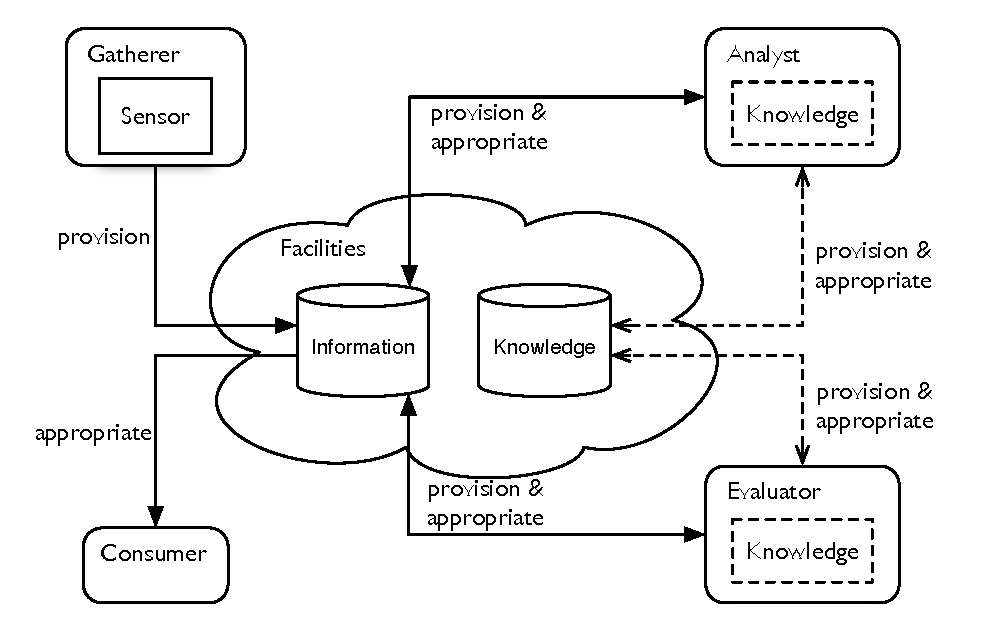
\includegraphics[width=\linewidth]{gfx/Prov_and_app_sys_diag}
\caption[Participatory sensing as a provision and appropriation system]{Participatory sensing as a provision and appropriation system. Dotted arrows represent optional actions for that role.}\label{fig:psys}
\end{figure}

\section{IAD Analysis}

Given participatory sensing as a provision and appropriation system, we can use the \ac{IAD} framework analyse, develop, and evaluate it. 
The \ac{IAD} is split into nine areas of analysis (\autoref{fig:iad}). 
The left side of the framework looks at what the resource and the community using it is like, and rules which have been created for resource and institution management. 
The middle section deals with where interactions occur and who these interactions are between. 
The right-hand side observes what the outcomes are and evaluates them.

Our use of the \ac{IAD} in the section is split into three parts.
Firstly we provide an analysis of a participatory sensing system using the left-hand side of the framework, looking at resource and community characteristics and rules-in-use. 
Secondly we propose a new set of rules-in-use to address each of Ostrom's principles for sustainable institutions. 
Finally we use the observational and evaluative aspects on the right of the \ac{IAD} framework to evaluate our proposed system.
The final part of this section addresses the issue of supply of such an institution.

\begin{figure}
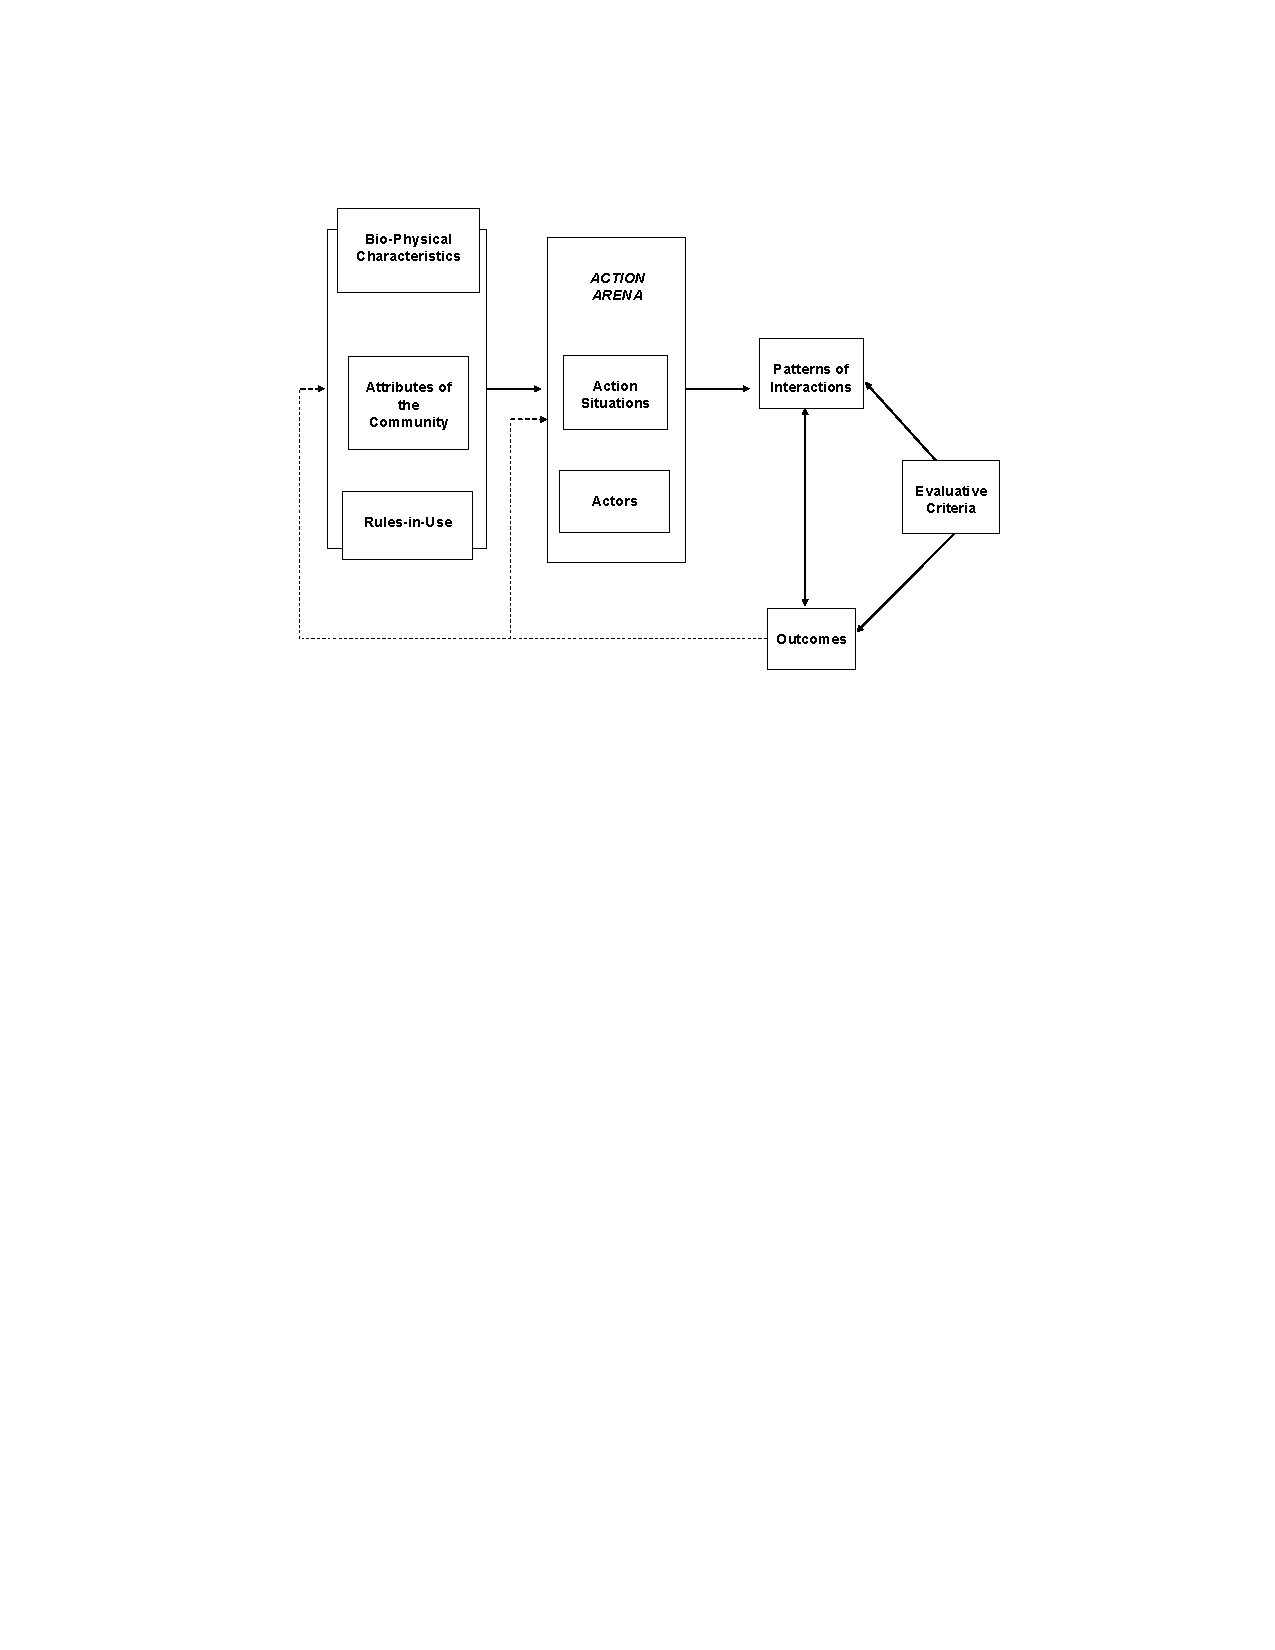
\includegraphics[width=\linewidth]{gfx/IAD.pdf}
\caption[Institutional Analysis and Development Framework]{Institutional Analysis and Development Framework~\protect\cite[p.44]{Ostrom2007a}}\label{fig:iad}
\end{figure}

We now present this analysis of participatory sensing as a provision and appropriation system. 
Following the \ac{IAD} framework we discuss the characteristics of the information and knowledge gathered through sensing as a resource (bio-physical characteristics), the community of individual actors involved in the sensing process (attributes of the community), and how institutional rules are or could be created (rules-in-use).

\subsection{Bio-Physical Characteristics}

Typically this area is concerned with the physical attributes of the resource, in terms of \emph{flow} and \emph{facility}. This distinction separates the resource units (\emph{flow}) from where they are stored and generated (\emph{facility}). In order to deal with the complexity of information and knowledge \citeasnoun{Ostrom2003} put forward an alternative method, considering \emph{ideas}, \emph{artifacts} and \emph{facilities}. 
In this framework, \emph{ideas} are data, information and knowledge in intangible form; \emph{artifacts} are the expression of ideas into tangible, observable form; and \emph{facilities} store artifacts and make them available. 
As intangible objects, \emph{ideas}, by definition, cannot be represented within a computational system---they must be expressed into files, databases or algorithms to be used. In this form they are then \emph{artifacts}. Therefore we treat \emph{ideas} as a resource flow external to the system, and instead manage the tangible derivative works from them: \emph{artifacts}.
%However, in a computational system \emph{ideas} can be ignored. It is impossible for data, information or knowledge to exist in such a system in intangible form. 
%Therefore \emph{ideas} are a resource flow external to the system we are considering.

In participatory sensing, the \emph{artifacts} are raw sensor data,
contextualised sensor information, algorithms for the analysis of data, and
rich information generated from these algorithms. Some of these artifacts will
be protected by copyright law, and this will affect what control the
organisation is able to have over them. The status of data and information (as
we have defined them) with regards to copyright is currently ambiguous,
traditionally it was not copyrightable, however databases are
copyrightable~\citep{Miller2008}. This copyright protection is important as it
affects how easily the organisation can protect its assets. Bad protection
limits the ability of the organisation to prevent \emph{forks}\footnote{A \emph{fork} is when a new organisation is formed from a copy of one repository of information or knowledge.} of the
information. This affects the excludability of the artifacts, as while one may
be able to exclude access to one database, if the information can be freely
copied elsewhere then this control is lost. It has become prevalent in the age
of digital information that when individuals feel there will be no or little
chance of punishment for sharing information, they do so on a large
scale~\citep[pp.\ 62--66]{Lessig2004}.

The \emph{facilities} constitute how the data, information and knowledge are
stored. A suitable facility depends on the properties of the resource (for
example, where this storage is physically located, \ie\ under whose control it
is) and who is willing to underwrite its costs.  In existing 
participatory-sensing applications the initiator, evaluators and/or analysts provide this
infrastructure and pay for it. Alternatives would be distributed or peer-to-peer 
databases where a set of individuals cooperatively provide infrastructure
and bear that cost (perhaps being compensated by those who cannot contribute).
A peer-to-peer system could be one where each individual looks after their own
data and responds to requests for it (cf. Global Sensor
Network~\citep{Aberer2006} and Open Mustard Seed~\citep{Hardjono2014}), or a
robust replicated system where every user has a copy of the whole data set
(cf. decentralised version-control system Git\footnote{http://git-scm.com} and
crypto-currency Bitcoin\footnote{http://bitcoin.org}), or anywhere between
these extremes.  We may also have different facilities for different artifact
types within a single organisation if the artifact quantity and transitivity
differ.

We can furthermore consider computational resources as facilities. Evaluators
and analysts use their knowledge (\ie\ algorithms) with the information stored
in the facility to generate new information. This process requires
computational resources which are provided by the evaluator or analyst
themselves. Alternatively participants could provision resources or share
costs for this computation. The commodification of computational resources
makes this very easy to achieve in practice as, for example, computing power
and storage space can be purchased on a metered basis from cloud providers,
preventing the need for large capital outlays.

\subsection{Attributes of the Community}

To identify the community for the knowledge commons, \citeasnoun{Ostrom2007a} begin by assessing information users, information providers and information policymakers. 
\emph{Users} appropriate information, \emph{providers} constitute both providers of artifacts and facilities, and \emph{policymakers} are those who partake in the organisational governance. 
Each of these groups contain multiple sub-groups, each with different interests and agendas.

The \emph{users} in participatory sensing are those appropriating information in order to apply knowledge to it (\emph{evaluators} and \emph{analysts}) and those appropriating this derived data (\emph{consumers}). As in many cases consumers are also providers as they have a reciprocal relationship with the analysts.

\emph{Providers} constitute the users providing sensor information (\emph{gatherers}), users providing both information derived from knowledge and/or the knowledge itself (\emph{evaluators} and \emph{analysts}), and users providing infrastructure for \emph{facilities}. This is a diverse group which is likely to involve almost all users in the application. However it is also one of the most critical groups, as a lack of provision will be a key factor in the success of the organisation. Big data has shown us that the value of information is additive, often exponentially so, and gaining traction---a critical mass of providers---is important. 
We have seen in \autoref{sec:review} some methods for incentivising contribution.

Finally, \emph{policymakers} constitute a more diverse and abstract group of community decision makers. Any \emph{user} or \emph{provider} can be a \emph{policymaker}, but equally, membership of those groups is not a requirement. 
Currently many participatory-sensing applications have a very small number of predefined \emph{policymakers}, and this is in direct violation of Ostrom's third principle---that those affected by the rules can participate in their modification. 
Therefore we would like to see larger groups of decision makers like in Wikipedia and \ac{FOSS}. This does not mean that all \emph{policymakers} will have equal power (in terms of capability to enact change) however, policy making communities can be nested, as we see in social communities and the systems reviewed in \autoref{sec:review}.


\subsection{Rules-in-Use}

The rules-in-use dictate what users must, must not, or may do in an organisation. The \ac{IAD} breaks these rules down into three levels: operational, collective-choice and constitutional. Operational rules deal with day-to-day operations regarding the resource, who can provision and appropriate what, and when. 
Collective-choice rules determine how operational rules can be changed, and constitutional rules determine who can participate in collective-choice decisions and how collective-choice rules can be changed.

For a knowledge commons \citeasnoun{Ostrom2007a} advocate the creation of rules by allocating bundles of property rights, a method which has also been adopted for the Creative Commons licenses\footnote{http://creativecommons.org}. 
Seven rights were identified~\citep{Schlager1992}:
\begin{itemize}
\item \emph{Access}---The right to enter an area and enjoy non-subtractive benefits. Typically this right would be for physical access to the property, though this concept can be extended to information commons. 
In participatory sensing, access would grant the ability to browse or search the repository, but not to extract anything. This can be likened to browsing a library without the right to loan anything. 
\item \emph{Contribution}---The right to contribute artifacts to the repository, or right of provision. This can be discriminated by the type of information/knowledge being contributed. 
\item \emph{Extraction}---The right to obtain artifacts, or right of appropriation. 
As with contribution this could be discriminated by information/knowledge type, for example only certain experts may be allowed to extract sensor information, but everyone can extract the information generated by these experts.
\item \emph{Removal}---The right to remove one's artifacts from the resource.
\item \emph{Management/Participation}---``The right to regulate internal use patterns and transform the resource by making improvements"~\cite[p.52]{Ostrom2007a}. 
The first part of this right is a collective-choice right, but the second part is also applied at the operational level. 
Management of the resource could involve pruning, aggregating or compressing information in order to keep facility costs down.
\item \emph{Exclusion}---``The right to determine who will have access, contribution, extraction and removal rights and how those rights may be transferred"~\cite[p.53]{Ostrom2007a}. 
This is a collective-choice right which controls the level of access for users of the resource. 
\item \emph{Alienation}---``The right to sell or lease extraction, management/participation, and exclusion rights"~\cite[p.53]{Ostrom2007a}. In this definition the sale of a right prohibits the seller from utilising that right once it is transferred. Therefore it is not a right which is particularly applicable to information commons.
\end{itemize}

With these rights we can make rules to describe the operational and most of the collective-choice levels of many organisations managing information and knowledge. Rights give users the institutional \emph{power}, \emph{permission} and/or \emph{obligation} to take actions within the context of a knowledge commons. We can formalise these relationships to write rules which are machine readable, such that agents can understand when they are permitted or obliged to perform actions, and when someone has broken the rules~\citep{Artikis2009}.

%\subsubsection*{Action Arena}

%The action arena encapsulates all the situations where interactions occur in the organisation. These action situations can be on different levels of the rule hierarchy, and on different scales (\ie\ local or global). In our case we see provision and appropriation on multiple levels as action situations (as illustrated in Figure~\ref{fig:psysex}). We also see action situations emerge around organisational actions such as access control and collective choice.

\section{Formal Characterisation}\label{sec:formalchar}

Having analysed participatory sensing as a knowledge commons, we can now begin to formally characterise such a system. \citeasnoun{Pitt2012b} used the \ac{EC}~\citep{Kowalski1986} and Institutionalised Power~\citep{Jones1996} to formally characterise a resource-allocation system and address six of \possessivecite{Ostrom1990} eight principles. 
We follow the same methodology, applying it instead to a provision and appropriation system with multiple resource types.

\autoref{fig:psysex} illustrates the participatory-sensing provision and appropriation system with multiple levels of information and knowledge. 
The same actions, \emph{provision} and \emph{appropriate}, can be used for several different resource types. 
As well as those shown in the diagram, facilities and institutions can be provisioned. 
We assume that we are able to distinguish between each of these resource types and thus tailor rules. In our representation we use simple predicates to make these distinctions.

\begin{figure}
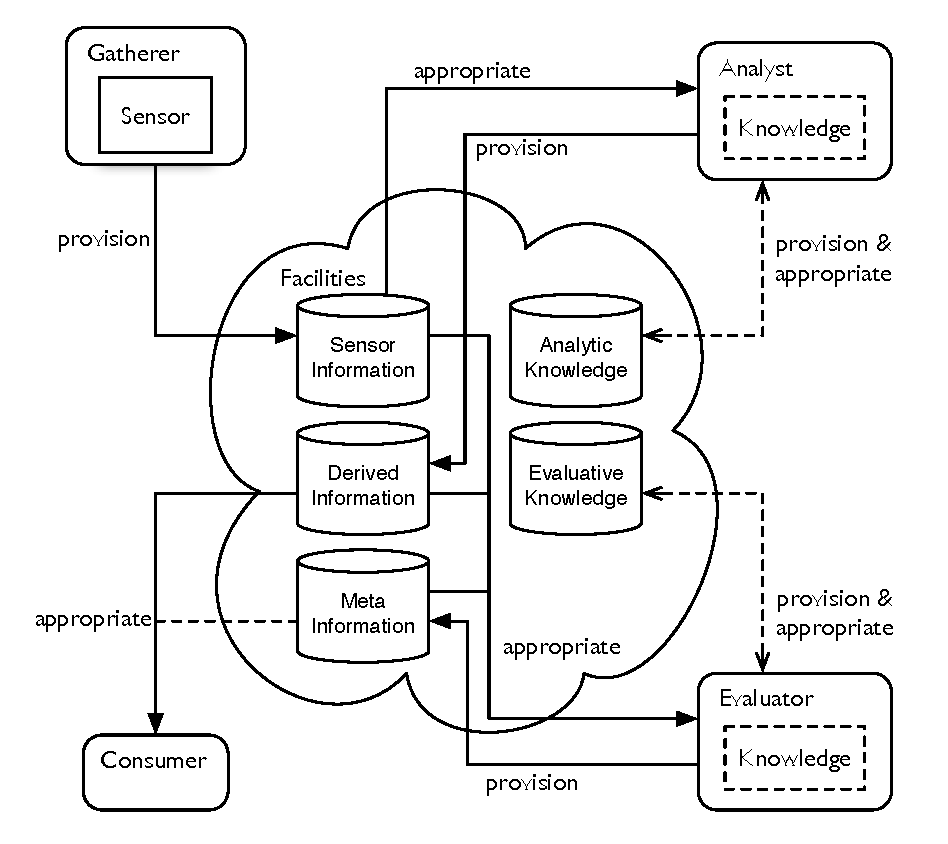
\includegraphics[width=\linewidth]{gfx/Prov_and_app_sys_diag_expanded}
\caption[Participatory sensing as a provision and appropriation with multiple types of information and knowledge.]{Participatory sensing as a provision and appropriation system with multiple types of information and knowledge. Raw information from sensors is provisioned then knowledge is used to generate multiple different types of information from this. Dotted arrows represent optional actions for that role.}\label{fig:psysex}
\end{figure}

%\subsubsection{Provision of an Institution}

%The first action which must be performed is the provision of rules-in-use for the organisation. We call a set of rules-in-use an institution. The agent providing the institution then assumes the role of \emph{initiator}.

%Within a participatory sensing application several organisations can co-exist. A new organisation is created when an agent \emph{provisions} an institution. The institution is the set of rules-in-use which the organisation will be following. By providing the institution the provisioning agent assumes the role of \emph{initiator}.

%Once the institution has been provisioned agents can join and being contributing to the resource. How they can do this will depend on the rules-in-use in the institution. We will now discuss how an institution can satisfy Ostrom's principles and formalise the rules required to do this.

\subsection{The Event Calculus and Institutionalised Power}\label{sec:ecprimer}

For this formalisation we wish to use a language which is able to represent and reason about action, agency, social constraints, and change. 
We continue with the \ac{EC}, as we are extended the specification from \citeasnoun{Pitt2012b}. Additionally, its clarity of exposition and executable specification are useful for this task.

The \ac{EC} is a logical formalism for representing and reasoning about actions or events and their effects, based on a many-sorted first-order predicate calculus. 
An \ac{EC} specification consists of an \emph{action description} which includes axioms that define: action occurrences, using $\mathsf{happensAt}$ predicates; the effects of actions, using $\mathsf{initiates}$ and $\mathsf{terminates}$ predicates; and the values of \emph{fluents}, using $\mathsf{initially}$ and $\mathsf{holdsAt}$ predicates. 
\autoref{table:ec} summarises \ac{EC} predicates which we use in our specification. 
Variables start with an upper case letter and are assumed to be universally quantified. Note that the underscore `\_' denotes
the anonymous variable which can stand for (be unified with) any value. 
Predicates, function symbols and constants start with a lowercase letter. 
\emph{Fluents} are properties which can have different values at different points in time.

\begin{table}[htbp]
\caption{Main Predicates  of the Event Calculus.}\label{table:ec}
\begin{center}
\renewcommand{\arraystretch}{0.9}
\setlength\tabcolsep{3pt}
\begin{tabular}{llcc}
\hline\noalign{\smallskip}
\multicolumn{1}{c}{\textbf{Predicate}} & \multicolumn{1}{c}{\textbf{Meaning}}  \\
\noalign{\smallskip}
\hline
\noalign{\smallskip}
$\mathit{Act} \,\, \mathsf{happensAt} \,\, T $ & Action $\mathit{Act}$ occurs at time $T$  \\[2pt]
$\mathsf{initially}$ $\mathit{F \val V}$ & The value of fluent $F$ is $V$ at time $0$  \\[2pt] 
$\mathit{F \val V} \,\, \mathsf{holdsAt} \,\, T$ & The value of fluent $F$ is $V$ at time $T$ 
\\[2pt] 
$\mathit{Act} \,\, \mathsf{initiates} \,\, F \val V \,\, \mathsf{at} \,\, T$ & The occurrence of action $\mathit{Act}$ at time $T$ \\ 
& initiates a period of time for which \\
& the value of fluent $F$ is $V$ \\[2pt] 
$\mathit{Act} \,\, \mathsf{terminates} \,\, F \val V \,\, \mathsf{at} \,\, T$ & The occurrence of action $\mathit{Act}$ at time $T$ \\
& terminates a period of time for which \\
& the value of fluent $F$ is $V$  \\
\hline
\end{tabular}
\end{center}
\end{table}

In order to represent and reason about permissions and access control within an institution we need a formalisation of \emph{institutionalised power}~\citep{Jones1996}. 
This term refers to the feature of institutions whereby designated agents, often acting in specific roles, are empowered, obliged or permitted to perform certain actions which in turn may modify certain institutional facts. 
In \ac{EC} we formalise these powers as fluents which indicate whether an agent has or had a specific power at a time.

An institutionalised power for an agent to perform an action signifies that
the institution has granted the agent the power that performing the designated
action will lead to a change in institutional state. The absence of this power
does not preclude the agent from perform this action however, it just means
that, as the institution does not recognise it as a valid action, it will not
result in the same change in institutional state as when the empowered agent
did the action. This power differs from physical capability, as one can still
perform an action when one is not empowered to do so, but the reverse is also
true, that one could be empowered to do something that one is not able to do.

Permission represents that an agent has been explicitly permitted to perform
an action by the institution. This is subtly different to power, as one can
have power but not permission. In this case performing the action will still
change institution state (as the agent was empowered), but may have later
repercussions.

Obligations specify actions which \emph{ought} to be performed. An agent with
an obligation to perform an action should perform that action to avoid
sanctions from the institution for non-compliance. They can often be used to
define protocol. For example a polling period for a vote can be defined by
setting an obligation for when the ballot must be closed.

To take an example of voting in an election. The state will
give \emph{permission} for a subset of the population to vote. However, the
people are not empowered to do so until they receive a valid polling card. At
the polling station, the staff are \emph{obliged} to give a citizen a voting
slip should they be presented with a valid polling card, and the time is
within the allowed voting period. With this slip they are then
\emph{empowered} to cast a vote, and performing the action of ticking a box
now counts as a valid vote in the election.

Should the staff fail in their obligation, and give a voting slip without
seeing a valid polling card, they may empower someone to vote who does not
have permission. The vote will still count, despite them not being permitted
to vote.

Alternatively, if someone arrived too late to the polling station they cannot
be given a voting slip, and therefore would not have the \emph{power} to vote,
despite having \emph{permission}.

Finally, someone could create their own voting slip, mark a cross on it, and
attempt to vote with it. They could still perform the voting action, however,
having not been correctly \emph{empowered}, the vote would not count, as the
counting process should identify an incorrect voting slip (provided it is not
produced to look the same as a valid one). This is an example of
performing an action without empowerment.

Institutionalised power therefore provides fine-grained and rich method of
describing the ways in which the rules of an institution are administered. It
has been argued (by \citet{Artikis2009a}) that being about to express these
powers is vital to be able to properly specify open systems governed by
institutional rules. Therefore we use this formalisation in our specification.

\subsection{Addressing Ostrom's principles}
%
%Having thoroughly analysed participatory sensing as a knowledge commons we now look at the provision of such a system. To do this we address \possessivecite{Ostrom1990} eight principles and discuss how they can be satisfied.

\citeasnoun{Pitt2012b} demonstrated that six of Ostrom's principles could be axiomatised for a resource-allocation problem. There are several differences between this problem and our provision and appropriation system. 
Therefore, we follow the same methodology but modify the axioms where appropriate. 
Their resource-allocation problem deals with an exogenous resource system, and as such does not deal with \emph{provisions} by agents. With an endogenous provision and appropriation system we must extend the specification to accommodate provision of resources.
%In resource-allocation systems there is a physical resource which is accessed through appropriations, while in our case the agents interact with provisions as well as appropriations. 
Furthermore, resource allocation deals with scarce, highly excludable resources, meaning that  one agent's appropriation excludes another agent from doing the same. 
In the case of information and knowledge, a key feature which we identified in \autoref{sec:commons}, is the lack of scarcity and excludability. 

The formal characterisation consists of a set of actions which agents can perform in the action arena of the participatory-sensing application, a set of fluents which describe the state of the system at discrete time points, and rules which describe how the agents' actions affect the fluents. Through this characterisation we enumerate how certain rules can satisfy some of Ostrom's principles, and may lead to certain outcomes. The rules are sourced from both social systems that we have reviewed and from technical solutions which are available for the virtual domain. \autoref{table:agact} lists agent actions, \autoref{table:fluents} lists fluents and \autoref{table:predicates} lists the
predicates and function symbols.

\begin{table}
\centering
\caption{Agent actions}\label{table:agact}
\begin{tabular}{ l | p{0.6\textwidth}}
\hline
Action & Description \\
\hline
$\m{provision}(A,I,\m{Obj})$ & Agent $A$ provisions object $\m{Obj}$ to institution $I$. \\
$\m{appropriate}(A,I,\m{Obj})$ & Agent $A$ appropriates object $\m{Obj}$ from institution $I$. \\
$\m{apply}(A,I,\m{Role})$ & Agent $A$ applies for the role $\m{Role}$ in institution $I$. \\
$\m{assign}(G,A,I,\m{Role})$ & Gatekeeper agent $G$ assigns the role of $\m{Role}$ in institution $I$ to agent $A$. \\
$\m{report}(M,A,I,\m{Reason})$ & Monitor agent $M$ reports agent $A$ in institution $I$ for the reason given by $\m{Reason}$. \\
$\m{appeal}(A,I,S)$ & Agent $A$ appeals the sanction level $S$ in institution $I$. \\
$\m{uphold}(C,A,I,S)$ & Head agent $C$ upholds the appeal by agent $A$ for the sanction level $S$ in institution $I$.
\end{tabular}
\end{table}
%
\begin{table}
\centering
\caption{Fluents}\label{table:fluents}
\begin{tabular}{ l | p{0.20\textwidth} | p{0.45\textwidth}}
\hline
Fluent & Values & Description \\
\hline
$\m{role\_of}(A,I,\m{Role})$ & \bool & $\true$ iff agent $A$ has the role of $\m{Role}$ in institution $I$. \\
$\m{provided}(A,I,\m{Obj})$ & \bool & $\true$ iff agent $A$ successfully provisioned $\m{Obj}$ to institution $I$. \\
$\m{appropriated}(A,I,\m{Obj})$ & \bool & $\true$ iff agent $A$ successfully appropriated $\m{Obj}$ from institution $I$. \\
$\m{applied}(A,I,\m{Role})$ & \bool & $\true$ iff agent $A$ successfully made an application for the role $\mathit{Role}$ in institution $I$. \\
$\m{acMethod}(I,\m{Role})$ & \{$\m{none}$, $\m{attribute}$, \newline$\m{discretionary}$, $\m{vote}$\} & Specifies the access control method for the role $\m{Role}$ in institution $I$ \\ 
$\m{appLimit}(I,\m{Role},\m{Rtype})$ & $($\integer$, \m{time})$ & The current rate limit on appropriations of the resource type $\m{Rtype}$ for the role $\m{Role}$ in institution $I$. Value is a two-tuple of number of appropriations over a discrete time period.\\
$\m{review\_score}(A,I)$ & $[0..1]$ & A rating of the agent $A$'s provisions to the institution $I$.\\
$\m{score\_threshold}(I)$ & $[0..1]$ & The threshold of provision quality required by the institution $I$.\\
$\m{appealed}(A,I,S)$ & \bool & $\true$ iff agent $A$ has made an appeal over the sanction level $S$ in institution $I$. \\
$\m{sanction\_level}(A,I)$ & \integer & The current sanction level of agent $A$ in institution $I$. \\
$\m{offences}(A,I)$ & \integer & The number of offences committed by agent $A$ in institution $I$. \\
$\m{adrMethod}(I)$ & $\{\m{arbitration},$\newline$\m{mediation},$\newline$\m{negotiation},\ldots\}$ & Specifies the dispute resolution method used in institution $I$. \\
$\m{licenceReq}(I)$ & $\{\m{none},\m{copyleft},$\newline$\ldots\}$ & Specifies the required licence for artifacts in institution $I$. \\
$\m{licence}(\m{Obj})$ & $\{\m{none},\m{copyleft},$\newline$\ldots\}$ & Gives the current licence type of artifact $\m{Obj}$. \\
$\B{pow}(A,\m{Action})$ & \bool & Agent $A$ has the institutionalised power to perform action $\m{Action}$ \\
$\B{per}(A,\m{Action})$ & \bool & Agent $A$ has the institutionalised permission to perform action $\m{Action}$ \\
$\B{obl}(A,\m{Action})$ & \bool & Agent $A$ is obliged to perform action $\m{Action}$ \\
\end{tabular}
\end{table}

\begin{table}
\centering
\caption{Predicate/Function Symbols}\label{table:predicates}
\begin{tabular}{ p{0.25\textwidth} | p{0.25\textwidth} | p{0.4\textwidth}}
\hline
Predicate/Function & Values/Range & Description \\
\hline
$\m{type}(\m{Obj})$ & \{$\m{sensor\_information}$, $\m{derived\_information}$, $\m{meta\_information}$, $\m{analytic\_knowledge}$, $\m{evaluative\_knowledge}$\} & Determines the artifact type of $Obj$. \\
$\m{countAppropriations}(\newline A,I,R,T1,T2)$ & \integer & Counts the number of appropriations by agent $A$ of resources of type $R$ in institution $I$ between times $T1$ and $T2$. \\
$\m{countProvisions}(\newline A,I,R,T1,T2)$ & \integer & Counts the number of provisions by agent $A$ of resources of type $R$ in institution $I$ between times $T1$ and $T2$. \\
$\m{derivedFrom}(\newline S,Alg,O)$ & \bool & $\true$ iff artifact $O$ was derived from artifact $S$ using $Alg$. \\
\end{tabular}
\end{table}

\subsubsection*{Principle 1: Clearly defined boundaries}

Defining boundaries for a digital resource is much easier than with physical resources. Firstly, the resource facility is not a pre-existing physical area, it is a virtual portal where the information and knowledge are stored. Access to the resource is much easier to control due to the availability of authentication mechanisms (\eg\ public key infrastructure, identity management, etc.) which allow the verification of users accessing the resource. 
Taking open-source software as an example, the facilities (the version control system, bug/issue tracker and mailing list) have fine grained access control, preventing unauthorised access to the resource. 

This access control can be implemented in a distributed system using a role-based system. 
In addition to the operational user roles for participatory sensing we add roles for institutional tasks, in this case an agent with the role of \emph{gatekeeper}. 
This role empowers this agent to assign roles according to the specified access-control method for the institution. An agent who applies for a role can be subsequently assigned to the role by the \emph{gatekeeper} provided the conditions of entry for the chosen access control method are satisfied. 

\mbox{\parbox{.95\columnwidth}{
\begin{tabbing}
\hspace*{.5cm}\=\hspace*{.5cm}\=\hspace*{.5cm}\=\kill
$\m{apply}(A,I,\Role) \initiates \m{applied}(A,I,\Role)=\true \pad$ at $\pad T \pad \leftarrow$ \\[0mm]
\>$\B{pow}(A, \m{apply}(A,I,\Role))=\true \holdsAt T$ \\
$\B{pow}(A, \m{apply}(A,I,\Role))=\true \holdsAt T \pad \leftarrow$ \\[0mm]
\>$\roleof(A,I,\Role)=\false \holdsAt T$ \\
$\m{assign}(G,A,I,\Role) \initiates \roleof(A,I,\Role)=\true \pad$ at $\pad T \pad \leftarrow$ \\[0mm]
\>$\B{pow}(G, \m{assign}(G,A,I,\Role))=\true \holdsAt T$ \\
$\B{pow}(G,\m{assign}(G,A,I,\Role))=\true \holdsAt T \pad \leftarrow$ \\[0mm]
\>$\m{applied}(A,I,\Role)=\true \holdsAt T \pad \land$ \\
\>$\m{acMethod}(I,\Role)=\m{discretionary} \holdsAt T \pad \land$ \\
\>$\roleof(G,I,\m{gatekeeper})=\true \holdsAt T$
\end{tabbing}
}}

The axioms above give the example of discretionary assignment, where the gatekeeper can decide whether to assign a role or not. 
An Agent $A$ performing the $\m{apply}$ action initiates a period of time during which the fluent $\m{applied}(A,I,\Role)$ is $\true$ if
it is empowered to perform that action; it is empowered to perform that action if the agent does not already occupy this role.
Similarly, an agent $G$ can make the institutional fact (fluent) true that an agent $A$ is assigned to a role $\Role$ if
it is empowered to perform the $\m{assign}$ action. This is the case if agent $A$ has applied for the role, agent $G$ occupies
the role of gatekeeper, and the access-control method is discretionary.

Note that we could also use attribute-based access control, where the gatekeeper may only assign the role if the applicant satisfies certain conditions. 
We could allow agents to vote on new applicants, or, if we want more open access to certain roles, we can compel the gatekeeper to assign a role to all applicants:

\mbox{\parbox{.95\columnwidth}{
\begin{tabbing}
\hspace*{.5cm}\=\hspace*{.5cm}\=\hspace*{.5cm}\=\kill
$\B{obl}(G, \m{assign}(G,A,I,\Role))=\true \holdsAt T \pad \leftarrow$ \\
\>$\Role=\m{gatherer} \pad \land$ \\ 
\>$\m{applied}(A,I,\Role)=\true \holdsAt T \pad \land$ \\
\>$\m{acMethod}(I,\Role)=\m{none} \holdsAt T \pad \land$ \\
\>$\roleof(G,I,\m{gatekeeper})=\true \holdsAt T$

\end{tabbing}
}}

Using roles we can define who will be \emph{empowered}, \ie\ have the right, to provision and appropriate certain resources, according to \autoref{fig:psysex}.

\mbox{\parbox{.95\columnwidth}{
\begin{tabbing}
\hspace*{.5cm}\=\hspace*{.5cm}\=\hspace*{.5cm}\=\kill
$\B{pow}(A, \provision(A,I,\Obj))=\true \holdsAt T \pad \leftarrow$ \\
\>$\roleof(A,I,\m{gatherer})=\true \holdsAt T \pad \land$ \\
\>$\m{type}(\Obj)=\m{sensor\_information}$ \\ 

$\B{pow}(A, \provision(A,I,\Obj))=\true \holdsAt T \pad \leftarrow$ \\
\>$\roleof(A,I,\m{analyst})=\true \holdsAt T \pad \land$ \\
\>$\m{type}(\Obj)=\m{derived\_information}$ \\

$\B{pow}(A, \provision(A,I,\Obj))=\true \holdsAt T \pad \leftarrow$ \\
\>$\roleof(A,I,\m{evaluator})=\true \holdsAt T \pad \land$ \\
\>$\m{type}(\Obj)=\m{meta\_information}$ 
\end{tabbing}
}}

The axioms for appropriation have the same structure, simply changing the \emph{provision} action to \emph{appropriation} and the role and resource type where applicable. \autoref{fig:psysex} specifies which roles can appropriate each resource type.

\subsubsection*{Principle 2: Congruence between appropriation and provision rules and local conditions}

The appropriation and provision rules must be relevant for the local conditions, and therefore are often quite application-specific. These rules cover time, place, technology and quantity of resource units appropriated or provisioned. The principle is typically violated when the rules cause over-regulation of an abundant resource, or under-regulation of a scarce one.

In participatory sensing, scarcity may arise in access to the resource, for example through an excessive quantity of requests going to the facility. 
One method of dealing with such congestion would be to rate limit requests. 
If we take an example of a consumer appropriating road traffic information from the facility, an incorrectly implemented rate-limit could severely limit the usefulness of the resource. 
As the nature of resource usage in this case is bursty (large number of requests in one go when route planning, then very few for a period of time afterwards), a quota system of $x$ requests per minute is extremely more restrictive than $60 \times 24 \times x$ requests per day, despite corresponding to the same overall quota.

Rate limits can be expressed as follows:

\mbox{\parbox{.95\columnwidth}{
\begin{tabbing}
\hspace*{.5cm}\=\hspace*{.5cm}\=\hspace*{.5cm}\=\kill
$\B{pow}(A, \m{appropriate}(A,I,\m{Obj}))=\true \holdsAt T \pad \leftarrow$ \\
\>$\m{type}(\m{Obj})=\m{Rtype} \pad \land$ \\ 
\>$\m{role\_of}(A,I,\m{Role})=\true \holdsAt T \pad \land$ \\
\>$\m{appLimit}(I,\m{Role},\m{Rtype})=(\m{Limit},\m{Period}) \holdsAt T \pad \land$ \\
\>$\m{countAppropriations}(A,I,\m{Rtype},T-\m{Period},T)<\m{Limit}$ 
\end{tabbing}
}}

In \citeasnoun{Pitt2012b} this principle is addressed by looking at when it is appropriate to demand resources. Here, the patterns of interaction are likely to be more free-form. However in some applications we may want to force a more symmetric relationship to compel agents to contribute to the resource:

\mbox{\parbox{.95\columnwidth}{
\begin{tabbing}
\hspace*{.5cm}\=\hspace*{.5cm}\=\hspace*{.5cm}\=\kill
$\B{pow}(A, \m{appropriate}(A,I,\m{Obj}))=\true \holdsAt T \leftarrow$ \\
\>$\m{countProvisions}(A,I,\m{Rtype},0,T)=P \pad \land$ \\
\>$\m{countAppropriations}(A,I,\m{Rtype},0,T) \leq P$ 
\end{tabbing}
}}

\subsubsection*{Principle 3 : Collective-choice arrangements}

``Most individuals affected by the operational rules can participate in modifying the operational rules" -- This is certainly not the case in current participatory-sensing applications. 
To achieve this, a framework is required to allow users to propose and agree on new rules and rule changes in the context of the application. 
Many such frameworks exist for human organisations, and some have been formalised to be usable for agent systems~\citep{Artikis2004}, including robust voting mechanisms~\citep{Pitt2005a}. 

\citeasnoun{Pitt2012b} formulate a voting mechanism for collective-choice arrangements through effective enfranchisement of members of the institution. This enfranchisement is achieved by empowering agents to vote and granting an entitlement associated with this right, ensuring a correct result is declared from a ballot. 
This entitlement is implemented as an obligation for a particular agent to declare the result of a vote according to an agreed-upon winner-determination method. 
This general voting system is fit for purpose across many domains, indeed it is just a formalisation of protocols used in many social systems~\citep{Pitt2005a}, and so we can adopt it as-is for this domain.

An issue remains, though, of how or whether agents can make reasoned decisions about rules, let alone create new rules, without human intervention. This problem has been explored with the implementation of the game of Nomic played by agents~\citep{Holland2013}. 
Normative synthesis~\citep{Morales2013} offers an approach to the generation of rules. 
We can use the concepts of learning, self-simulation and self-awareness to provide some reasoning about the consequences of rules.

\subsubsection*{Principle 4: Monitoring}

Monitoring can be implemented, provided sufficient auditing capabilities are available~\citep{Pitt2012b}. Wikipedia sets a good example here: all users are able to monitor each other through the edit history, which gives a fine-grained breakdown of what has been contributed and by whom. 
In technical systems, this auditing can be done via a log of institutional actions performed by agents. This creates a narrative, like the ones which can be processed with the \ac{EC}, and the process of monitoring is simply looking for actions which are performed when the actor did not have the permission to perform that action at the time.

Effective monitoring can occur in several different ways. 
Firstly, some systems can be designed such that monitoring is a side-effect arising from normal use. 
\citeasnoun{Ostrom1990} observed this in fisheries which allocated areas of a lake to different individuals on a rota. 
If an individual, upon arriving in their allotted zone, found someone else using it they would obviously have detected the violation of the rules and be able to report it. 
Secondly, individuals can be incentivised to monitor for violations. Unlike in the first case this involves some additional effort on the individual's part. 
This incentivisation can be in the form of a reward for finding violations or payment for performing audits. 
Finally, the institution can arrange for an independent third party to monitor the system, and pay for this by collecting contributions from members.

In the participatory-sensing scenario our access-control procedures provide protection over access to the resource, therefore monitoring is more concerned with the content of provisions: The quality of information and knowledge provided, and whether a user is permitted to provision a particular artifact. 
These requirements touch on different concepts and thus need to be handled differently. 

In the case of the quality of provisioned information and knowledge, the actions of \emph{evaluators} can be a form of monitoring. 
Meta information provisioned by \emph{evaluators} can provide indications of the trustworthiness and accuracy of sensor information, derived information and even other meta information (see \autoref{fig:psysex}). 
This process is akin to review, rating and trust systems seen in e-commerce and other online applications. Provided that there are \emph{evaluators} provisioning this kind of information in the institution, this is a form of side-effect monitoring. 
Incentives can also be created to encourage more provision of meta information.

% EC
We may assign a \emph{monitor} role to an agent who is required to monitor for low-quality provisions. 
To do this, they can simply look for information provisioned by \emph{evaluators} that suggests an agent's data is below some quality threshold. 
If this is the case, it will trigger a report of that agent (indeed, the monitor may even be obliged to report the offence):

\mbox{\parbox{.95\columnwidth}{
\begin{tabbing}
\hspace*{.5cm}\=\hspace*{.5cm}\=\hspace*{.5cm}\=\kill
$\m{report}(M,A,I,O) \initiates \m{monitored\_offence}(A,I)=O \pad at \pad T \pad \leftarrow$ \\[0mm]
\>$\B{pow}(M, \m{report}(M,A,I,O))=\true \holdsAt T$ \\
$\B{pow}(M,\m{report}(M,\_,I,\_))=\true \holdsAt T \pad \leftarrow$ \\[0mm]
\>$\m{role\_of}(M,I,\m{monitor})=\true \holdsAt T$ \\
$\B{obl}(M,\m{report}(M,A,I,\m{baddata}))=\true \holdsAt T \pad \leftarrow$ \\[0mm]
\> $\m{review\_score}(A,I)=S \holdsAt T \pad \land$ \\
\> $\m{score\_threshold}(I)=\m{Thres} \holdsAt T \pad \land$ \\
\> $S<\m{Thres}$
\end{tabbing}
}}

The other concern, provision of artifacts when the individual does not have the permission to, is more difficult to monitor. There are two possible malicious actions here which we may want to monitor: An agent provisioning an artifact which has already been provisioned previously; and an agent provisioning an artifact which was generated by another, but has not been provisioned to this institution. In both cases the agent acts maliciously in order to gain benefits of provision without having to generate an artifact legitimately. 

However, any open system facing the problem of  non-compliant behaviour has to consider the related problems: how 
are these actions detectable, and if so, is it even worthwhile to monitor? It has been shown (\eg\ \citet{Balke2013}) that the cost of monitoring
can outweigh the benefits of preventing or punishing non-compliant behaviour. This can be particularly acute in any system
with endogenous resources, where the cost of monitoring has to be `paid for' from the same common pool resource that is
itself being monitored.

%The questions which we must answer are: Are these actions desirable, are these actions detectable and if so, is it worthwhile to monitor for this?

%We may also ask, who will monitor? Finding violations of the rules in a large application will require a large number of motivated agents to search the action history. While individuals will see a benefit from increases in monitoring level, up to a point~\citep{Pitt2012c}, they can also receive the same benefit if someone else does the monitoring. Therefore this scenario is set up as a prisoner's dilemma, and intervention will be required to resolve it.

%If we wish to choose the route of collective monitoring we can utilise the organisation's facilities and take fees from members to pay for monitoring. An alternative is to take a less formal monitoring approach a rely on trust and reputation to find malicious actors, similar to how we see some online marketplaces operating. In this case the evaluators act as monitors, and as the meta-information they generate also has value then this mechanism can motivate a high level of monitoring.

% Monitoring as by product, 

\subsubsection*{Principle 5: Graduated sanctions}

In order to have graduated sanctions, we require multiple levels of punishment. 
Firstly, as we have control over the system's boundaries through access control, we can implement temporary and permanent banishment as possible sanctions. 
Secondly we can revoke certain provision and/or appropriation rights. Finally, if there exists some form of micro-payment system, we can levy fines against members. 
Therefore, given that we have several forms of sanction which differ in both context and severity, we should be able to implement graduated sanctions. 

\citeasnoun{Pitt2012b} use a sanction level which increases on each new offence for that agent.
At higher sanction levels a nominated agent (in this case a role of \emph{head} assumes this responsibility) is empowered (and may be obliged) to impose stronger sanctions. 
This method assumes equal weight to each offence, though we may define some offences which can cause multiple level increases. 

\subsubsection*{Principle 6: Conflict-resolution mechanisms}

In Ostrom's work this principle was mainly used to deal with conflict due to ambiguities arising from the way that rules were written. Rules in a computational system (if written correctly) should not have any ambiguities, so theoretically there should be no need for this principle.

However, as we have collective-choice arrangements, we have a system which has a rule which says that the rules should be changeable. \citeasnoun{Suber1990} hypothesised that such a system will inevitably lead to paradox or gaps in the rule-set. 
Given this, the question is whether to give agents recourse to retrospectively claim for losses due to such issues through conflict-resolution.

%Given this, the question is whether this is something which simply should be fixed after it is detected, through the use of collective choice, or some recourse should be provided retrospectively through conflict-resolution.

In \citeasnoun{Pitt2012b} Alternative Dispute Resolution (ADR) is used as a fast, cheap and effective conflict-resolution mechanism. A simple appeals procedure is given, allowing one to appeal sanctions. A more complete specification of an ADR protocol is given in \citeasnoun{Pitt2012}. 
We will simply give an overview of the semantics of the appeal process, and the method of deciding whether an appeal is valid and should be upheld. How one argues one's case is beyond the scope of this work, but there are several approaches to choose from.

For example, the agent occupying the requisite role ($\m{head}$) is empowered to sanction another agent if an offence has been reported (see Principle 4), and this action increases the sanction level against this agent.

\mbox{\parbox{.95\columnwidth}{
\begin{tabbing}
\hspace*{.5cm}\=\hspace*{.5cm}\=\hspace*{.5cm}\=\kill
$\m{sanction}(H,I,A,O) \initiates \m{sanction\_level}(A,I)=S1 \pad$ at $\pad T \pad \leftarrow$ \\[0mm]
\>$\B{pow}(H, \m{sanction}(H,I,A,O))=\true \holdsAt T \pad \land$ \\
\>$\m{sanction\_level}(A,I)=S \holdsAt T \pad \land$ \\
\>$S1=S+1$ \\
$\B{pow}(H,\m{sanction}(H,I,A,O))=\true \holdsAt T \pad \leftarrow$ \\[0mm]
\>$\m{role\_of}(H,I,\m{head})=\true \holdsAt T \pad \land $ \\
\>$\m{monitored\_offence}(A,I)=O \holdsAt T $
\end{tabbing}
}}

An agent may appeal against its sanction level:

\mbox{\parbox{.95\columnwidth}{
\begin{tabbing}
\hspace*{.5cm}\=\hspace*{.5cm}\=\hspace*{.5cm}\=\kill
$\m{appeal}(A,I,S) \initiates \m{appealed}(A,I,S)=\true \pad$ at $\pad T \pad \leftarrow$ \\[0mm]
\>$\B{pow}(A, \m{appeal}(A,I,S))=\true \holdsAt T $ \\
$\B{pow}(A,\m{appeal}(A,I,S))=\true \holdsAt T \pad \leftarrow$ \\[0mm]
\>$\m{role\_of}(A,I,\_)=\true \holdsAt T \pad \land$ \\
\>$\m{sanction\_level}(A,I)=S \holdsAt T $
\end{tabbing}
}}

The \emph{head} may then lower the sanction level if the appeal is successful. If the ADR method for the institution is arbitration, then the \emph{head} agent, can decide the outcome of the appeal process itself.

\mbox{\parbox{.95\columnwidth}{
\begin{tabbing}
\hspace*{.5cm}\=\hspace*{.5cm}\=\hspace*{.5cm}\=\kill
$\m{uphold}(H,A,I,S) \initiates \m{sanction\_level}(A,I)=S1 \pad$ at $\pad T \pad \leftarrow$ \\[0mm]
\>$\B{pow}(H, \m{uphold}(H,A,I,S))=\true \holdsAt T \pad \land$ \\
\>$\m{sanction\_level}(A,I)=S \holdsAt T \pad \land$ \\
\>$S1=S-1$ \\
$\B{pow}(H,\m{uphold}(H,A,I,S))=\true \holdsAt T \leftarrow$ \\[0mm]
\>$\m{role\_of}(H,I,\m{head})=\true \holdsAt T \pad \land$ \\
\>$\m{appealed}(A,I,S)=\true \holdsAt T \pad \land$ \\
\>$\m{adrMethod}(I)=\m{arbitration} \holdsAt T $
\end{tabbing}
}}

An appeal which is upheld could also initiate review and retraction of the monitored offence (axioms not specified here).

% Maybe mention Pitt2012 conflict resolution or *-justice.

\subsubsection*{Principle 7: Minimal recognition of rights to organise}

This principle states that external entities should not interfere with the rule-making capabilities of the organisation. \citeasnoun{Heller1998} wrote that over regulation leads to under-use of a common-pool resource, which he called a `Tragedy of the Anti-commons'. The use of copyright law has the capability of subverting the internal rules of an information commons.

If users attempt to assert their intellectual property rights in participatory-sensing applications they could gain more rights than the organisation initially permitted them with, or gain the power to prevent others performing actions. For example an analyst may determine that information he generates and provisions is his intellectual property. 
If an evaluator then wants to appropriate this information and generate some meta information about it, this could be seen as a derivative work, and therefore require the permission of the analyst. 
Scenarios like this need to be prevented as they stifle productivity (evaluators will be cautious about what information they appropriate for fear of infringement) and undermine the authority of the organisation.

Luckily, there has already been significant success in dealing with these issues. Licenses have been used to ensure that certain rights are released when information is provisioned. In open-source software Copyleft~\citep{Stallman1999} is an example which uses copyright law to its advantage to provide additional benefits in return. The Creative Commons\footnote{http://creativecommons.org} licenses simplify the process of inferring what rights one has regarding specific content. Care must be taken to choose appropriate licenses for the different forms of information and knowledge generated from the sensing application.

In order to protect itself, an institution may require that contributions are licensed in a particular way:

\mbox{\parbox{.95\columnwidth}{
\begin{tabbing}
\hspace*{.5cm}\=\hspace*{.5cm}\=\hspace*{.5cm}\=\kill
$\B{per}(A, \m{provision}(A,I,\m{Obj}) \holdsAt T \pad \leftarrow$ \\[0mm]
\>$\m{licenceReq}(I)=L \holdsAt T \pad \land$ \\
\>$\m{licence}(Obj)=L \holdsAt T$ \\
\end{tabbing}
}}

We can also formalise aspects of some open-source licences. For example: the right to redistribute; the right to read source code (which we interpret as an obligation to provision any knowledge which copylefted information is derived with); and the obligation to provision any derivative works back to the institution(s) it originated from.

\mbox{\parbox{.95\columnwidth}{
\begin{tabbing}
\hspace*{.5cm}\=\hspace*{.5cm}\=\hspace*{.5cm}\=\kill
$\m{provision}(A,I,\m{Obj}) \initiates \B{obl}(A, \m{provision}(A,I,\m{Alg})) \pad$ at $\pad T \pad \leftarrow$ \\
\>$\m{derivedFrom}(\_,\m{Alg},\m{Obj})=\true \pad \land$ \\
\>$\m{licence}(\m{Obj})=\m{copyleft} \holdsAt T \pad \land$ \\
\>$\m{provisioned}(\_,I,\m{Alg})=\false \holdsAt T$ \\
$\B{per}(A,\m{provision}(A,\_,\m{Obj}) \holdsAt T \pad \leftarrow$ \\
\>$\m{licence}(\m{Obj})=\m{copyleft} \holdsAt T$ \\
$\m{provision}(A,\m{I2},\m{Obj}) \initiates \B{obl}(A, \m{provision}(A,I,\m{Obj})) \pad$ at $\pad T \pad \leftarrow$ \\
\>$\m{derivedFrom}(\m{Source},\_,\m{Obj})=\true \pad \land$ \\
\>$\m{licence}(\m{Source})=\m{copyleft} \holdsAt T \pad \land$ \\
\>$\m{provisioned}(\_,I,\m{Source})=\true \holdsAt T \pad \land$ \\
\>$I \neq \m{I2}$ \\
\end{tabbing}
}}

Note that the presence of a derivative work can only be detected once it is provisioned elsewhere. Additionally, what constitutes \emph{derivedFrom} can be difficult to pinpoint in many cases~\citep{Lessig2004}.

%\subsubsection*{Principle 8: Nested enterprises}

%Splitting a complex organisation into multiple layers of nested enterprises helps to simplify decision making in each layer. Figure~\ref{fig:psysex} shows how, when decomposed, our participatory sensing provision and appropriation system contains multiple nested operations. These operations refer to particular action situations, e.g. the collection and provision of sensor information, and they each have some independence from the system as a whole. 

\section{Evaluation}

We now move on to the evaluative aspects of the \ac{IAD}. We perform this evaluation with respect to current participatory sensing applications and our proposed self-organising approach based on Ostrom's design principles. We first look at possible outcomes arising from applications, then determine a set of criteria to evaluate them with.

\subsection{Outcomes}

We have talked of some current outcomes seen in participatory-sensing applications, namely enclosure and inequity. 
This analysis should help us understand why we see these, but we will also look at other potential outcomes we may observe from different organisational approaches. 

\paragraph{Enclosure}
What we see in often participatory sensing and other applications based around information collection is the enclosure of the database. 
The data collector wants to keep the information to try and derive as much value from it themselves as possible. 
This is firstly inefficient; when data is made open much more total value is derived than any individual could achieve by themselves~\citep{Shadbolt2012}. 
Secondly, it deprives the original information provider, the user, from their own property. 

\paragraph{Access}
The opposite to the negative outcome of enclosure is access. 
This has a beneficial effect of having an information and knowledge resource where there was none before. 
The benefits of access increase the more open the information is.

\paragraph{Equity}
Equity and inequity are outcomes based on the fairness of the allocation of the resource, in terms of information and knowledge availability. Fairness can be evaluated in several different ways, many of which are subjective. We can use a more objective measure by assessing whether each user is compensated according to the value of their input to the system. 

%Many participatory sensing applications fail to gain significant traction because gatherers don't believe them to be meritorious. They 

\paragraph{Pollution}
The insertion of incorrect information can affect the quality of the resource. 
This information could be contributed accidentally, \eg\ a gatherer, whose sensor is faulty, provisioning information, or maliciously, \eg\ doctoring information to gain a competitive edge~\citep{Oreskes2010}. 
The \emph{evaluator's} role can be to validate information and guard against pollution,
for example through trust and reputation systems, or redundancy in the information gathering process (this approach has been used to combat pollution in peer-to-peer systems~\citep{Kamvar2003,Costa2007}).

\paragraph{Degradation and Depletion}
These outcomes are caused by either the removal of information, or insufficient provision of new information. 
These relate to the endurance of a system. They will occur either when the system does not react to changing external or internal conditions,  or if the system evolves into a `bad' state, causing participation to be no longer worthwhile for some agents. 
Lack of reactivity to changing conditions is likely to be caused by a lack of flexibility in the institution, either by not having mechanisms in place for reacting, or such mechanisms being blocked by entrenched interests or inappropriate decision-making processes~\citep{North1990}. 
Similarly `bad' states can be caused by malicious groups of agents manipulating the institution for short-term benefit.

\subsection{Evaluative Criteria}

Finally, to access the efficacy of the organisational structure on the outcomes of the system we specify a set of evaluative criteria. 
We evaluate outcomes and participant's interactions with measurable values, allowing objective comparison of systems and organisations. 
We take general criteria applied to knowledge commons, as proposed by \citeasnoun{Ostrom2007a}, describe how we can measure them, and then discuss the effect we expect our framework will have on the values of the criteria. 
These criteria are: increase in knowledge, sustainability and preservation, participation standards, economic efficiency and equity through fiscal equivalence.

A successful participatory-sensing application should lead us to have increased knowledge, in terms of more information derived from a large pool of sensor information. 
However we may also see an improvement in the knowledge being applied to the information by analysts and evaluators.
% E.g. machine learning ensembles.
For example, for some machine learning problems, better results can be achieved by combining several algorithms together as an \emph{ensemble}~\citep{Opitz1999}.
%In academia it is generally accepted that open collaboration can improve the quality of knowledge generated. 
Allowing participants to share their knowledge and then allow others to modify and improve it is an efficient way of increasing knowledge, and one which could be leveraged in participatory sensing. Therefore the increase in knowledge can be measured as the quantity and quality of information generated by the application.

% Quantity through incentivisation and participation. Quality through monitoring and evaluation.
Quantity of provision is achieved through high participation standards and incentivisation. 
In our survey we saw several methods of incentivising provision, and our self-organising approach makes several of these methods available as rules-in-use. 
Quality is maintained through effective monitoring. 
We have discussed how monitoring can be achieved in our system and be responsive to increases in malicious actions using principles four and five. 
The differentiating factor between our proposed framework and other participatory-sensing applications is the pool of knowledge available in parallel with information. This permissive sharing of knowledge, allowing for iterative improvements by many disparate contributors, is an effective method for the increase of knowledge, as demonstrated by academia, \ac{FOSS} and Wikipedia.

Sustainability and preservation of the organisation can be measured in terms of how long the system endures before participation ceases or falls below a certain threshold (where the system is not longer economically viable). 
To achieve sustainability it must be possible to meet the needs of the majority of participants over the long term, and also to react to changes in conditions. 
For example, combating a rise in malicious actors before the information pool becomes over-polluted. 

Linked to sustainability are participation standards. 
This relates to the number of participants in the system (and in each user role), as well as the level of contribution from each of those participants. Low levels of participation or asymmetric participation (\eg\ appropriating more than one provides) may be interpreted as free-riding, depending on the system's rules. 
Free-riding is a frequent negative behaviour in the commons and is likely to affect participation standards if not controlled.

% Reactivity better with self-org.
Through collective-choice, a self-organising institution should be more sustainable than dictatorial institutions, as each agent is properly enfranchised and is able to address any issues they have with the current rules. 
Equally effective self-organisation should imply good reactivity to changing conditions. 
However, we must consider the possible implications of inappropriate collective-choice procedures which can cause deadlocks. 
Voting mechanisms can be manipulated, or unrealistic win criteria may be required for the passing of motions~\citep{Conitzer2007,Pitt2011b}. 
In social systems we can identify these issues and attempt to work around them, but in computational systems collective choice will simply grind to a halt, 
unless we explicitly build in procedures to deal with this.
%Therefore, we must be careful in the supply of institutions that these issues are considered.

Participation standards can be maintained through both enfranchisement and incentivisation. 
Participatory sensing also has a promotional aspect to it, which helps to gain and maintain participation. 
For example, OpenSignal largely relies on media publicity to attract users. 
This is an aspect where open access to information helps. 
Users are more likely to engage with an organisation if they initially get something for free. 
This gives them an idea of the product and its value, and may then lead to a more active role in the institution. 
Both Wikipedia and \ac{FOSS} projects work based on this concept, however they only need a very small proportion of appropriators to provision to the knowledge pool. 

It is also possible to measure the economic efficiency of a participatory-sensing application. We can count the utility generated by the consumers through the use of information appropriated and compare this to the total cost of maintaining the resource. This cost contains facility costs and the individual costs incurred by participants in information gathering and processing.

% Will self-org be more efficient than centralised.
If we compare centralised with self-organising approaches according to this metric, it is difficult to determine which will perform better. 
A self-organising institution requires additional facilities for the execution of the governance layer of the application. 
Our position is however, that a self-organising institution will be able to generate more value under the same conditions, due to the outcomes we have discussed, than a dictatorial one. 
In order to be more efficient overall, this increase in generated value must outweigh the additional operating costs.

Finally, we can assess equity through fiscal equivalence. 
This is a measure of the ratio of effort put in, versus benefit extracted from a system. 
An observation from other knowledge commons is that consumers often benefit for little or no effort (\eg\ Wikipedia, open-access publishing, FOSS). However this benefit is not at a cost to the knowledge providers---in these examples consumption by others usually benefits the providers, helping them achieve fiscal equivalence---but is a form of redistributional equity. In participatory sensing there is not such a strong benefit to information providers from its consumption so we focus more on fiscal equivalence and equality.

Together, these criteria offer a way of measuring the quality of the outcomes
of a knowledge commons. Later, we will derive metrics from these criteria for
our model of participatory sensing.

\section{Supply of a Participatory Sensing commons}

\newacro{GSN}{Global Sensor Network}
\newacro{OMS}{Open Mustard Seed}

The final question we must answer is how we can enable the supply of an institution as we have described for participatory sensing. 
Our requirements are a platform which can be easily deployed and is capable of providing a technical means to administer the rules-in-use needed to satisfy Ostrom's principles, and therefore create a sustainable institution around the participatory sensing application. 
We review the suitability of existing platforms for use with our framework, and advocate one which we believe fits our criteria best.


There exist several platforms specifically for the deployment of participatory sensing. 
CarTel~\citep{Hull2006} is a centralised system designed to accommodate heterogeneous sensor data and provides a web-based portal for data access. 
SenseWeb~\citep{Kansal2007} provides a shared resource for concurrent sensing applications with a centralised coordinator directing information acquisition and aggregation. 
It enables users demanding information to provide incentives for those who are able to provide it. 
\ac{GSN}~\citep{Aberer2006} is a peer-to-peer network of sensor nodes which can advertise and respond to queries for data streams across the network. 
G-Sense~\citep{Perez2010} is a platform which uses a hybrid architecture to achieve scalability, using local centralised hubs which collaborate with a global peer-to-peer network. 
\citeasnoun{Demirbas2010} leverage Twitter as infrastructure for information provision using encoded tweets.

In general, similar to what we found in our review in \autoref{sec:review}, these platforms are dealing with a particular technical challenge of participatory sensing. 
Therefore, these platforms do not specify how rules for membership, provision and appropriation quantities, monitoring and accountability can be implemented. 
In peer-to-peer platforms such as \ac{GSN}, individuals may be able to control access to their own data by selectively honouring requests, however there is no governance over-sight to keep consistency and fairness. 
The use of Twitter as an independent third party infrastructure provider provides a more transparent operation, but sacrifices all control over access to the resource.

\ac{OMS}~\citep{Hardjono2014,Hardjono2014a} is an open-source project which aims to give users control over their data in the cloud through a technical architecture based on trust and the formation of self-organising groups. 
A key feature is a rule engine governing access to data on a per-user basis and explicit recognition of governance as a key factor in the system.
Such a platform could enable the formation of institutions for participatory sensing with transparency over information access and use, but also with overrides for users. 
The \ac{OMS} architecture is peer-to-peer, enabling sharing of facility costs by design, and offering scalability and data privacy. 
%For these reasons we see \ac{OMS} as an implementation avenue for our framework.

%TODO may concluding statement.

\section{Summary}\label{sec:conclude}

In this chapter we have firstly described a framework for participatory sensing as a provision and appropriation system. We then gave a detailed analysis, using the \ac{IAD}, of this system to determine how it can be managed according as a knowledge commons, according to Ostrom's design principles. We adapted the axiomatisation of these principles, by \citet{Pitt2012b}, to be suitable for provision and appropriation in the knowledge commons. We then evaluated what kind of outcomes we can expect from such a commons in participatory sensing. Finally, we discussed how these electronic institutions may be deployed for participatory-sensing applications.

Our formalisation of institutional rules, specified in \ac{EC}, represents the formal characterisation phase of the \ac{SIC} methodology. Our evaluation thus far has only been hypothetical. In order to produce an objective evaluation we must create a computer model within which we can test these rules. The next two chapters address the technical challenge of this process.

% This paper has articulated the usefulness of the participatory-sensing paradigm and the shortfalls arising from the lack of consideration of the impact of governance in current applications in this area. 
% Our approach aims to find a method of democratising the large-scale aggregation of user-generated information, with participatory sensing as an example of this process. As these systems are digital, and often online, using electronic institutions and algorithmic governance enables us to bring both the enforcement of rules, as well as governance determining what the rules are, into one place. It also enables autonomous agents to interact with the governance layer along with human actors. In future work, we envision enabling this interaction through
% serious games and gamification, with an emphasis on the visualisation of the `state' of the common pool and the rule
% (see \citep{Bourazeri12} for an example using SmartMeters with energy as the common pool), and through
% design contractualism, whereby design decisions and governance models are manifested both in the code and in the interface
% \citep{Pitt12}.

% sec 2: participatory sensing is kc
%We have identified that participatory sensing entails the provision and appropriation of information and knowledge to a central pool by various individuals, and that this characterisation matches that of a knowledge commons~\citep{Hess2007}.  

%We identified that the flexibility of digital information and knowledge as goods results in a dilemma for creators. This dilemma is then likely to cause a tragedy of the commons, where less knowledge is available and, as a consequence, less knowledge is produced.
%Like with physical commons, successful commons in information and knowledge have been built with institutions which have been shown to satisfy Ostrom's principles for enduring institutions. Therefore we have proposed and formalised a form of algorithmic governance for participatory sensing in line with these principles.

%In Section~\ref{sec:commons} we introduced information and knowledge commons and showed that participatory sensing can be seen as one. 
%We then reviewed participatory sensing applications in Section~\ref{sec:review} identifying the issues of governance within them. 
%In this section we also reviewed successful knowledge commons in social systems which conform to Ostrom's principles. 
%The outcome of this review was that proper governance can overcome the tragedy of the commons, 
%Then in Section~\ref{sec:iad} we characterised participatory sensing as a provision and appropriation system and, using the IAD, formalised how such a system can be designed according to Ostrom's design principles for self-governing institutions. 
%This analysis includes a set of objective evaluative criteria which can be used to access the efficacy of a system and its governance.


% In summary, have made two main contributions, namely:
% \begin{itemize}
% \item Data clouds in open participatory-sensing applications can be construed as information and knowledge commons and thus characterised by provision and appropriation actions; and
% \item A system for access control (i.e. provision and appropriation) in participatory-sensing applications can be designed according to Ostrom's institutional design principles for self-governing institutions and formally specified in an action language.
% \end{itemize}
% We presented in Section~\ref{sec:commons} the literature on how information and knowledge can be seen as a commons, and, being a system with the purpose of gathering information in order to generate new knowledge, that participatory sensing enables the creation of information and knowledge commons. Following a review of participatory-sensing applications we were able to characterise a generic participatory-sensing application as a provision and appropriation system in Section~\ref{sec:iad}. We then formally defined a framework for the management of an information and knowledge commons in participatory sensing.

% We have two primary motivations for why such a framework is needed in this domain. 
% Firstly, through our review of participatory sensing in Section~\ref{sec:review}, we identified a lack of governance supplied for applications. Given that participatory sensing is a knowledge commons, appropriate governance, as stressed by \possessivecite{Ostrom1990} work, is important for its successful management. The success of certain knowledge commons such as Wikipedia and Free/Open-Source Software, which have been retrospectively shown to conform to the principles which Ostrom proposed, further reinforces this point. Thus, as information and knowledge is gathered more and more on the Internet, it is important that governance is supplied in order to fairly protect the interests of all involved parties and stakeholders.

% Secondly, the digitisation of information and knowledge has caused a shift in its properties as a good~\citep{Ostrom2003}. However, legal interpretations have not yet been fully updated to this new reality, leading to exploitative and restrictive consequences~\citep{Lessig2004}. We concluded that this gives the knowledge creator complete control over what class of good their knowledge falls in to, and leads to a dilemma where knowledge is enclosed for short-term benefits and a negative long-term outcome.

% With the presentation of this framework we are taking the first steps to the supply of institutional governance for managing information and knowledge commons in participatory-sensing applications.
% What remains to do is a quantitative comparison of the different rule permutations which can be instantiated on top of our framework and an objective comparison between centralised and community governance. 
% Our framework is flexible enough to be able to represent a centralised governance as well as the self-organising approach which is required for Ostrom's principles. 
% It is the aim of our future work to answer these questions.

% In conclusion, we have shown that consideration of governance and supply thereof is important in order to achieve the potential of the participatory-sensing paradigm. 
% By drawing on the management of the commons, we can create efficient and empowering institutions around information and knowledge resources, which can exploit the power of open data. 
% Additionally, given increasing concerns over data acquisition and data privacy in the digital age, our general representation of a system for the provision and appropriation of information could have applications beyond those which we have discussed here.